% This file was created (at least in part) by the script ParseMdtoLatex by Louis du Plessis
% (Available from https://github.com/taming-the-beast)

\documentclass[11pt]{article}
%%%%%%%%%%%%%%%%%%%%%%%%%%%%%%%%%%%%%%%%%%%%%%%%%%%%%%%%%%%%%%%
% DO NOT EDIT THIS FILE UNLESS YOU KNOW WHAT YOU ARE DOING!!! %
%%%%%%%%%%%%%%%%%%%%%%%%%%%%%%%%%%%%%%%%%%%%%%%%%%%%%%%%%%%%%%%

\usepackage[]{authblk}
\usepackage{graphicx}
\usepackage{color}
\usepackage{longtable}
\usepackage{hanging}
\usepackage{indentfirst}
\usepackage{setspace}
\usepackage{enumitem}
\usepackage{verbatim}
\usepackage{upgreek}
\usepackage{framed}
\usepackage{textcomp}
\usepackage{url}
\usepackage{soul}
\usepackage{amsmath, amsfonts,amssymb,mathrsfs}
\usepackage{fancyhdr}
\usepackage[compact]{titlesec}
\usepackage[T1]{fontenc}
\usepackage{lmodern}

\usepackage[backend=bibtex,hyperref=true,citestyle=authoryear,bibstyle=authortitle,firstinits=true,terseinits=true,doi=false,url=false,eprint=false,maxbibnames=10,maxcitenames=2]{biblatex}
\DeclareCiteCommand{\cite}
  {\usebibmacro{prenote}}
  {\usebibmacro{citeindex}%
   \printtext[bibhyperref]{\usebibmacro{cite}}}
  {\multicitedelim}
  {\usebibmacro{postnote}}

\DeclareCiteCommand*{\cite}
  {\usebibmacro{prenote}}
  {\usebibmacro{citeindex}%
   \printtext[bibhyperref]{\usebibmacro{citeyear}}}
  {\multicitedelim}
  {\usebibmacro{postnote}}

\DeclareCiteCommand{\parencite}[\mkbibparens]
  {\usebibmacro{prenote}}
  {\usebibmacro{citeindex}%
    \printtext[bibhyperref]{\usebibmacro{cite}}}
  {\multicitedelim}
  {\usebibmacro{postnote}}

\DeclareCiteCommand*{\parencite}[\mkbibparens]
  {\usebibmacro{prenote}}
  {\usebibmacro{citeindex}%
    \printtext[bibhyperref]{\usebibmacro{citeyear}}}
  {\multicitedelim}
  {\usebibmacro{postnote}}

\DeclareCiteCommand{\footcite}[\mkbibfootnote]
  {\usebibmacro{prenote}}
  {\usebibmacro{citeindex}%
  \printtext[bibhyperref]{ \usebibmacro{cite}}}
  {\multicitedelim}
  {\usebibmacro{postnote}}

\DeclareCiteCommand{\footcitetext}[\mkbibfootnotetext]
  {\usebibmacro{prenote}}
  {\usebibmacro{citeindex}%
   \printtext[bibhyperref]{\usebibmacro{cite}}}
  {\multicitedelim}
  {\usebibmacro{postnote}}

\DeclareCiteCommand{\textcite}
  {\boolfalse{cbx:parens}}
  {\usebibmacro{citeindex}%
   \printtext[bibhyperref]{\usebibmacro{textcite}}}
  {\ifbool{cbx:parens}
     {\bibcloseparen\global\boolfalse{cbx:parens}}
     {}%
   \multicitedelim}
  {\usebibmacro{textcite:postnote}}

\newcommand{\citep}{\parencite}
\newcommand{\citet}{\textcite}
\defbibheading{relevref}[\refname]{\section*{Relevant References}}

\renewcommand{\postnotedelim}{\iffieldpages{postnote}{\addcolon}{\addcomma\space}} 
\DeclareFieldFormat{postnote}{#1} 

\DeclareFieldFormat[article, inbook, incollection, inproceedings, patent, thesis, unpublished]{title}{#1}
\DeclareFieldFormat[article, inbook, incollection, inproceedings, patent, thesis, unpublished]{journaltitle}{\mkbibemph{#1}\nopunct}
\DeclareFieldFormat[article, inbook, incollection, inproceedings, patent, thesis, unpublished]{volume}{{#1}\addcolon} %puts volume number in parens
%\DeclareFieldFormat[article, inbook, incollection, inproceedings, patent, thesis, unpublished]{year}{\mkbibparens{#1}\nopunct} %puts year in parens

\DeclareFieldFormat[article, incollection, patent, thesis, unpublished]{pages}{{\nopp#1}}

\DeclareFieldFormat{sentencecase}{\MakeSentenceCase{#1}}

\renewbibmacro*{title}{%
  \ifthenelse{\iffieldundef{title}\AND\iffieldundef{subtitle}}
    {}
    {\ifthenelse{\ifentrytype{article}\OR\ifentrytype{inbook}%
      \OR\ifentrytype{incollection}\OR\ifentrytype{inproceedings}%
      \OR\ifentrytype{inreference}}
      {\printtext[title]{%
        \printfield[sentencecase]{title}%
        \setunit{\subtitlepunct}%
        \printfield[sentencecase]{subtitle}}}%
      {\printtext[title]{%
        \printfield[titlecase]{title}%
        \setunit{\subtitlepunct}%
        \printfield[titlecase]{subtitle}}}%
     \newunit}%
  \printfield{titleaddon}}

\DefineBibliographyStrings{english}{% various adjustments to common bib entry strings
urlseen = {Accessed:},% What goes in front of the date a URL was accessed/retrieved etc.
editor = {(Ed)},%Ed – no dot, in brackets
editors = {(Eds)},% Eds – no dot, in brackets
byeditor = {(Ed.)}}% ‘Edited by’ for edited works

\DeclareNameAlias{default}{last-first}

\renewbibmacro{in:}{}

\renewbibmacro{publisher+location+date}{
  \iflistundef{publisher}
    {}
    {\printlist{publisher}%
       {\addcomma\space}%
      \iflistundef{location}
        {}
        {\printlist{location}}%
    }
}

\DeclareBibliographyDriver{article}{%
\usebibmacro{bibindex}%
\usebibmacro{begentry}%
\usebibmacro{author/translator+others}%
\newunit\newblock
\printfield{year}%
\setunit{\labelnamepunct}\newblock
\usebibmacro{title}%
\newunit
\printlist{language}%
\newunit\newblock
\usebibmacro{byauthor}%
\newunit\newblock
\usebibmacro{bytranslator+others}%
\newunit\newblock
\printfield{version}%
\newunit\newblock
%\usebibmacro{in:}% %mit in:
\usebibmacro{journal}%
\newunit\newblock
\printfield{volume}%
\newunit\newblock
\usebibmacro{byeditor+others}%
\newunit\newblock
\usebibmacro{note+pages}%
\newunit\newblock
\iftoggle{bbx:isbn}
{}%
\newunit\newblock
\usebibmacro{doi+eprint+url}%
\newunit\newblock
\usebibmacro{addendum+pubstate}%
\newunit\newblock
\usebibmacro{pageref}%
\usebibmacro{finentry}}

\DeclareBibliographyDriver{inproceedings}{%
\usebibmacro{bibindex}%
\usebibmacro{begentry}%
\usebibmacro{author/translator+others}%
\newunit\newblock
\printfield{year}%
\setunit{\labelnamepunct}\newblock
\usebibmacro{title}%
\newunit
\printlist{language}%
\newunit\newblock
\usebibmacro{byauthor}%
\newunit\newblock
\usebibmacro{bytranslator+others}%
\newunit\newblock
\printfield{version}%
\newunit\newblock
%\usebibmacro{in:}% %mit in:
\usebibmacro{booktitle}%
\newunit\newblock
\printfield{volume}%
\newunit\newblock
\usebibmacro{byeditor+others}%
\newunit\newblock
\usebibmacro{publisher+location+date}%
\newunit\newblock
\usebibmacro{note+pages}%
\newunit\newblock
\usebibmacro{pageref}%
\usebibmacro{finentry}}

\DeclareBibliographyDriver{book}{%
\usebibmacro{bibindex}%
\usebibmacro{begentry}%
\usebibmacro{author/translator+others}%
\newunit\newblock
\printfield{year}%
\setunit{\labelnamepunct}\newblock
\usebibmacro{title}%
\newunit
\printlist{language}%
\newunit\newblock
\usebibmacro{byauthor}%
\newunit\newblock
\usebibmacro{bytranslator+others}%
\newunit\newblock
%\usebibmacro{in:}% %mit in:
\usebibmacro{booktitle}%
\newunit\newblock
\printfield{volume}%
\newunit\newblock
\usebibmacro{publisher+location+date}%
\newunit\newblock
\usebibmacro{note+pages}%
\newunit\newblock
\usebibmacro{pageref}%
\usebibmacro{finentry}}




\setlist{nolistsep}

\setlength{\evensidemargin}{0in}
\setlength{\headheight}{0in}
\setlength{\headsep}{0in}
\setlength{\oddsidemargin}{-0.25in}
\setlength{\paperheight}{11in}
\setlength{\paperwidth}{8.5in}
\setlength{\tabcolsep}{0in}
\setlength{\textheight}{9in}
\setlength{\textwidth}{7in}
\setlength{\topmargin}{0in}
\setlength{\topskip}{0in}
\setlength{\voffset}{0in}
\parskip = 0.15in
\pagestyle{plain}
\setlength{\parindent}{0cm}

\definecolor{citescol}{RGB}{194,101,1}
\definecolor{urlscol}{RGB}{0,150,206}
\definecolor{linkscol}{RGB}{149,0,207}
\definecolor{mycol}{RGB}{25,23,191}
\definecolor{outputcol}{RGB}{34,139,34}
\definecolor{tcol}{RGB}{165,0,14}


\DeclareMathAlphabet{\msfsl}{T1}{cmr}{m}{it}
\DeclareMathAlphabet{\msyf}{OMX}{pcr}{m}{it}
\newcommand{\alf}{\upalpha}
\newcommand{\hilight}[1]{\colorbox{yellow}{#1}}

\newcommand{\levelone}[1]{
\bigskip
\noindent{\LARGE{\textsc{#1}}}
\vspace {0.05in}
}

\newcommand{\leveltwo}[1]{
\bigskip
\noindent{\Large{\textit{#1}}}
\vspace {-1mm}
}

\newcommand{\descriptionhead}[1]{
\noindent{\textcolor{mycol}{\textbf{\textit{#1}}}}\\ \vspace{-7mm}
}

\newcommand{\dhead}[1]{
\noindent{\textbf{\textit{#1 --}}}
}



\newcommand{\exs}[1]{
\vspace{-4mm}
\begin{itemize}
\item #1 \\ \vspace{-8mm}
\end{itemize}
}

\newcommand{\nbo}[1]{{\color{red}{#1}}}


\newcommand{\stepbullet}{\noindent \textbullet \ }
\newcommand{\mi}[1]{\textbf{\textit{#1}}}


\newcommand{\levelthree}[1]{\textit{#1 --}}


%\bibliographystyle{apalike}
%\bibpunct[; ]{(}{)}{;}{a}{,}{;}


\usepackage[breaklinks]{hyperref}
\usepackage[all]{hypcap}
\hypersetup{colorlinks=true,linkcolor=linkscol,citecolor=citescol,urlcolor=urlscol}


\newcommand{\R}{\texttt{R} }
\newcommand{\TESS}{\texttt{TESS}}
\newcommand{\PBD}{\texttt{PBD}}
\newcommand{\DDD}{\texttt{DDD}}
\newcommand{\Laser}{\texttt{laser}}
\newcommand{\TreePar}{\texttt{TreePar}}
\newcommand{\diversitree}{\texttt{diversitree}}
\newcommand{\RevBayes}{\texttt{RevBayes}}
\newcommand{\Rev}{\texttt{Rev}}
\newcommand{\MrBayes}{\texttt{MrBayes}}
\newcommand{\BEAST}{\texttt{BEAST}}
\newcommand{\PhyloBayes}{\texttt{PhyloBayes}}
\newcommand{\PAML}{\texttt{PAML}}

\let\otheriint\iint
\let\iint\relax
\usepackage{ wasysym }

\usepackage{framed}
\usepackage[]{listings}
%\usepackage{fontspec}
\usepackage{placeins}
\usepackage{epstopdf}



\lstset{backgroundcolor=\color[rgb]{0.972,0.972,0.972},
		tabsize=4,
		rulecolor=,
        basicstyle=\scriptsize,
        upquote=true,
        aboveskip={1.5\baselineskip},
        columns=fixed,
        showstringspaces=false,
        extendedchars=true,
        breaklines=true,
        prebreak = \raisebox{0ex}[0ex][0ex]{\ensuremath{\hookleftarrow}},
        frame=single,
        showtabs=false,
        showspaces=false,
        showstringspaces=false,
        identifierstyle=\ttfamily,
        keywordstyle=\color[rgb]{0,0,1},
        commentstyle=\color[rgb]{0.133,0.545,0.133},
        stringstyle=\color[rgb]{0.627,0.126,0.941}
}

\definecolor{shadecolor}{RGB}{194,225,255}

\setlength{\tabcolsep}{5pt}
\setlength{\topmargin}{-0.4in}
\setlength{\headheight}{14.5pt}
\pagestyle{fancy}

\newcommand{\taha}[1]{{\textcolor{red}{[TAH comment: #1]}}} % TAH comment

\titlespacing{\section}{0pt}{*0}{*0}
\titlespacing{\subsection}{0pt}{*0}{*0}
\titlespacing{\subsubsection}{0pt}{*0}{*0}

\titleformat{\section}
  {\normalfont\Large\bfseries\color{mycol}}
  {\thesection}{1em}{}

\titleformat{\subsection}
  {\normalfont\large\bfseries\color{mycol}}
  {\thesubsection}{1em}{}

\titleformat{\subsubsection}
  {\normalfont\bfseries\color{mycol}}
  {\thesubsubsection}{1em}{}

% command for MrBayes command-line step
\newcommand{\cl}[1]{{\texttt{\textbf{#1}}}}

\newcommand{\colx}[1]{{\textcolor{tcol}{#1}}}

\newcommand{\mbcl}[1]{\exs{\cl{MrBayes > {#1}}}}

\newcommand{\rbprmt}{RevBayes > } 
\newcommand{\rbcl}[1]{\exs{\cl{\rbprmt{#1}}}}
\newcommand{\rbout}[1]{\exs{\cl{\textcolor{outputcol}{#1}}}}
\newcommand{\rbdn}{{\Large \symbol{126}}} % This makes a copy/pasteable tilde
\newcommand{\rbclml}[1]{\exs{\cl{\ \ \ \ \ \ \ \ \ \ \ {#1}}}}

% text box settings
% requires compiling w/ XeLaTeX
%\newfontfamily\listingsfont[Scale=1.0]{Courier New}
%\lstset{basicstyle=\listingsfont, columns=texcl}
%\defaultfontfeatures{Mapping=tex-text}


\makeatletter
\lst@CCPutMacro\lst@ProcessOther {"2D}{\lst@ttfamily{-{}}{-{}}}
\@empty\z@\@empty
\makeatother


\usepackage{tikz}

\setlength{\topmargin}{-0.4in}
\setlength{\headheight}{14.5pt}
\pagestyle{fancy}

\usepackage[breaklinks]{hyperref}
\usepackage[all]{hypcap}
\hypersetup{colorlinks=true,linkcolor=linkscol,citecolor=citescol,urlcolor=urlscol}

\definecolor{lg}{gray}{0.75}
\def\gcirc{{%
    \setbox0\hbox{$\fullmoon$}%
    \rlap{\hbox to \wd0{\hss{$\textcolor{lg}{\newmoon}$}\hss}}\box0
}}



% Add your bibtex library here
\addbibresource{master-refs}


%%%%%%%%%%%%%%%%%%%%
% Do NOT edit this %
%%%%%%%%%%%%%%%%%%%%
\begin{document}
\renewcommand{\headrulewidth}{0.5pt}
\headsep = 20pt
\lhead{ }
\rhead{\textsc {BEAST v2 Tutorial}}
\thispagestyle{plain}


%%%%%%%%%%%%%%%%%%
% Tutorial title %
%%%%%%%%%%%%%%%%%%
\begin{center}

	% Enter the name of your tutorial here
	\textbf{\LARGE Tutorial using BEAST v2.7.x}\\\vspace{2mm}

	% Enter a short description of your tutorial here
	\textbf{\textcolor{mycol}{\Large Skyline plots}}\\

	\vspace{4mm}

	% Enter the names of all the authors here
	{\Large {\em Nicola F. Müller and Louis du Plessis}}
\end{center}

Inference of past population dynamics using Bayesian Coalescent Skyline
and Birth-Death Skyline plots.

%%%%%%%%%%%%%%%%%
% Tutorial body %
%%%%%%%%%%%%%%%%%

\hypertarget{background}{%
\section{Background}\label{background}}

Population dynamics influence the shape of the tree and consequently,
the shape of the tree contains some information about past population
dynamics. The so-called Skyline methods allow to extract this
information from phylogenetic trees in a non-parametric manner. It is
non-parametric since there is no underlying system of differential
equations governing the inference of these dynamics. In this tutorial we
will look at two different methods to infer these dynamics from sequence
data. The first one is the Coalescent Bayesian Skyline plot
\citep{Drummond2005}, which is based on the coalescent model, and the
second one is the Birth-Death Skyline plot \citep{Stadler2013} based on
the birth-death model. The conceptual difference between the coalescent
and birth-death approaches lies in the direction of the flow of time. In
the coalescent, time is modeled to move backwards, from the present to
the past, while in the birth-death approach it is modeled to go
forwards. Two other fundamental differences are the parameters that are
inferred and the way sampling is treated. \clearpage

\hypertarget{programs-used-in-this-exercise}{%
\section{Programs used in this
Exercise}\label{programs-used-in-this-exercise}}

\hypertarget{beast2---bayesian-evolutionary-analysis-sampling-trees-2}{%
\subsubsection{BEAST2 - Bayesian Evolutionary Analysis Sampling Trees
2}\label{beast2---bayesian-evolutionary-analysis-sampling-trees-2}}

BEAST2 (\url{http://www.beast2.org}) is a free software package for
Bayesian evolutionary analysis of molecular sequences using MCMC and
strictly oriented toward inference using rooted, time-measured
phylogenetic trees. This tutorial is written for BEAST v2.7.x \citep{Bouckaert2014 Bouckaert2019}.

\hypertarget{beauti---bayesian-evolutionary-analysis-utility}{%
\subsubsection{BEAUti - Bayesian Evolutionary Analysis
Utility}\label{beauti---bayesian-evolutionary-analysis-utility}}

BEAUti2 is a graphical user interface tool for generating BEAST2 XML
configuration files.

Both BEAST2 and BEAUti2 are Java programs, which means that the exact
same code runs on all platforms. For us it simply means that the
interface will be the same on all platforms. The screenshots used in
this tutorial are taken on a Mac OS X computer; however, both programs
will have the same layout and functionality on both Windows and Linux.
BEAUti2 is provided as a part of the BEAST2 package so you do not need
to install it separately.

\hypertarget{tracer}{%
\subsubsection{Tracer}\label{tracer}}

Tracer (\url{http://beast.community/tracer}) is used to summarise the
posterior estimates of the various parameters sampled by the Markov
Chain. This program can be used for visual inspection and to assess
convergence. It helps to quickly view median estimates and 95\% highest
posterior density intervals of the parameters, and calculates the
effective sample sizes (ESS) of parameters. It can also be used to
investigate potential parameter correlations. We will be using Tracer
v1.7.x.

\hypertarget{r-rstudio}{%
\subsubsection{R / RStudio}\label{r-rstudio}}

We will be using \href{/href\%7Bhttps://www.r-project.org}{R} to analyze
the output of the Birth-Death Skyline plot.
\href{https://www.rstudio.com/}{RStudio} provides a user-friendly
graphical user interface to R that makes it easier to edit and run
scripts. (It is not necessary to use RStudio for this tutorial).
\clearpage

\hypertarget{practical-bayesian-and-birth-death-skyline-plots}{%
\section{Practical: Bayesian and Birth-Death Skyline
Plots}\label{practical-bayesian-and-birth-death-skyline-plots}}

In this tutorial we will estimate the dynamics of the Egyptian Hepatitis
C epidemic from genetic sequence data collected in 1993.

The aim of this tutorial is to:

\begin{itemize}

\item
  Learn how to infer population dynamics;
\item
  Get to know how to choose the set-up of a skyline analysis;
\item
  Get to know the advantages and disadvantages of the Coalescent
  Bayesian Skyline Plot and the Birth-Death Skyline.
\end{itemize}

\hypertarget{the-data}{%
\subsection{The Data}\label{the-data}}

The dataset consists of an alignment of 63 Hepatitis C sequences sampled
in 1993 in Egypt \citep{Ray2000}. This dataset has been used previously
to test the performance of skyline methods
\citep{Drummond2005 Stadler2013}.

With an estimated 15-25\%, Egypt has the highest Hepatits C prevalence
in the world. In the mid 20th century, the prevalence of Hepatitis C
increased drastically (see Figure \ref{fig:prevalence} for estimates).
We will try to infer this increase from sequence data.

The alignment file can be downloaded from the Taming the BEAST website
at \url{https://taming-the-beast.org/tutorials/Skyline-plots/} by
downloading the file \passthrough{\lstinline!hcv.nexus!} from the
left-hand panel, under the heading \textbf{Data}.

\begin{figure}
    \centering
    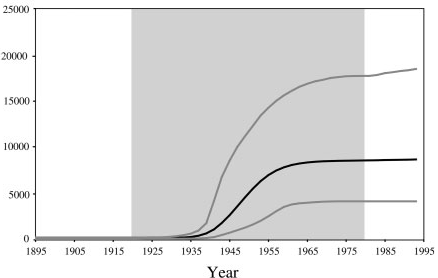
\includegraphics[width=0.500000\textwidth]{figures/Estimated_number_hcv.png}
    \caption{The growth of the effective population size of the Hepatitis C epidemic in Egypt \citep{Pybus2003}.}
    \label{fig:prevalence}
\end{figure}

\hypertarget{creating-the-analysis-files-with-beauti}{%
\subsection{Creating the Analysis Files with
BEAUti}\label{creating-the-analysis-files-with-beauti}}

We will use BEAUti to generate the configuration file for BEAST2 from
the sequence alignment.

\hypertarget{install-beast-2-packages}{%
\subsubsection{Install BEAST 2
packages}\label{install-beast-2-packages}}

While the coalescent-based Bayesian Skyline Plot is integrated in the
BEAST2 core, we need to install the BDSKY package, which contains the
Birth-Death Skyline model. Installation of packages is done using the
package manager, which is integrated into BEAUti.

\begin{framed}
Open the \textbf{BEAST2 Package Manager} by navigating to \textbf{File
\textgreater{} Manage Packages}.

Install the \textbf{BDSKY} package by selecting it and clicking the
\textbf{Install/Upgrade} button (Figure \ref{fig:install}).
\end{framed}

After the installation of a package, the program is on your computer,
but BEAUti is unable to load the template files for the newly installed
model unless it is restarted. So, let's restart BEAUti to make sure we
have the \textbf{BDSKY} model at hand.

\begin{framed}
Close the \textbf{BEAST2 Package Manager} and \textbf{\emph{restart}}
BEAUti to fully load the \textbf{BDSKY} package.
\end{framed}

\begin{figure}
    \centering
    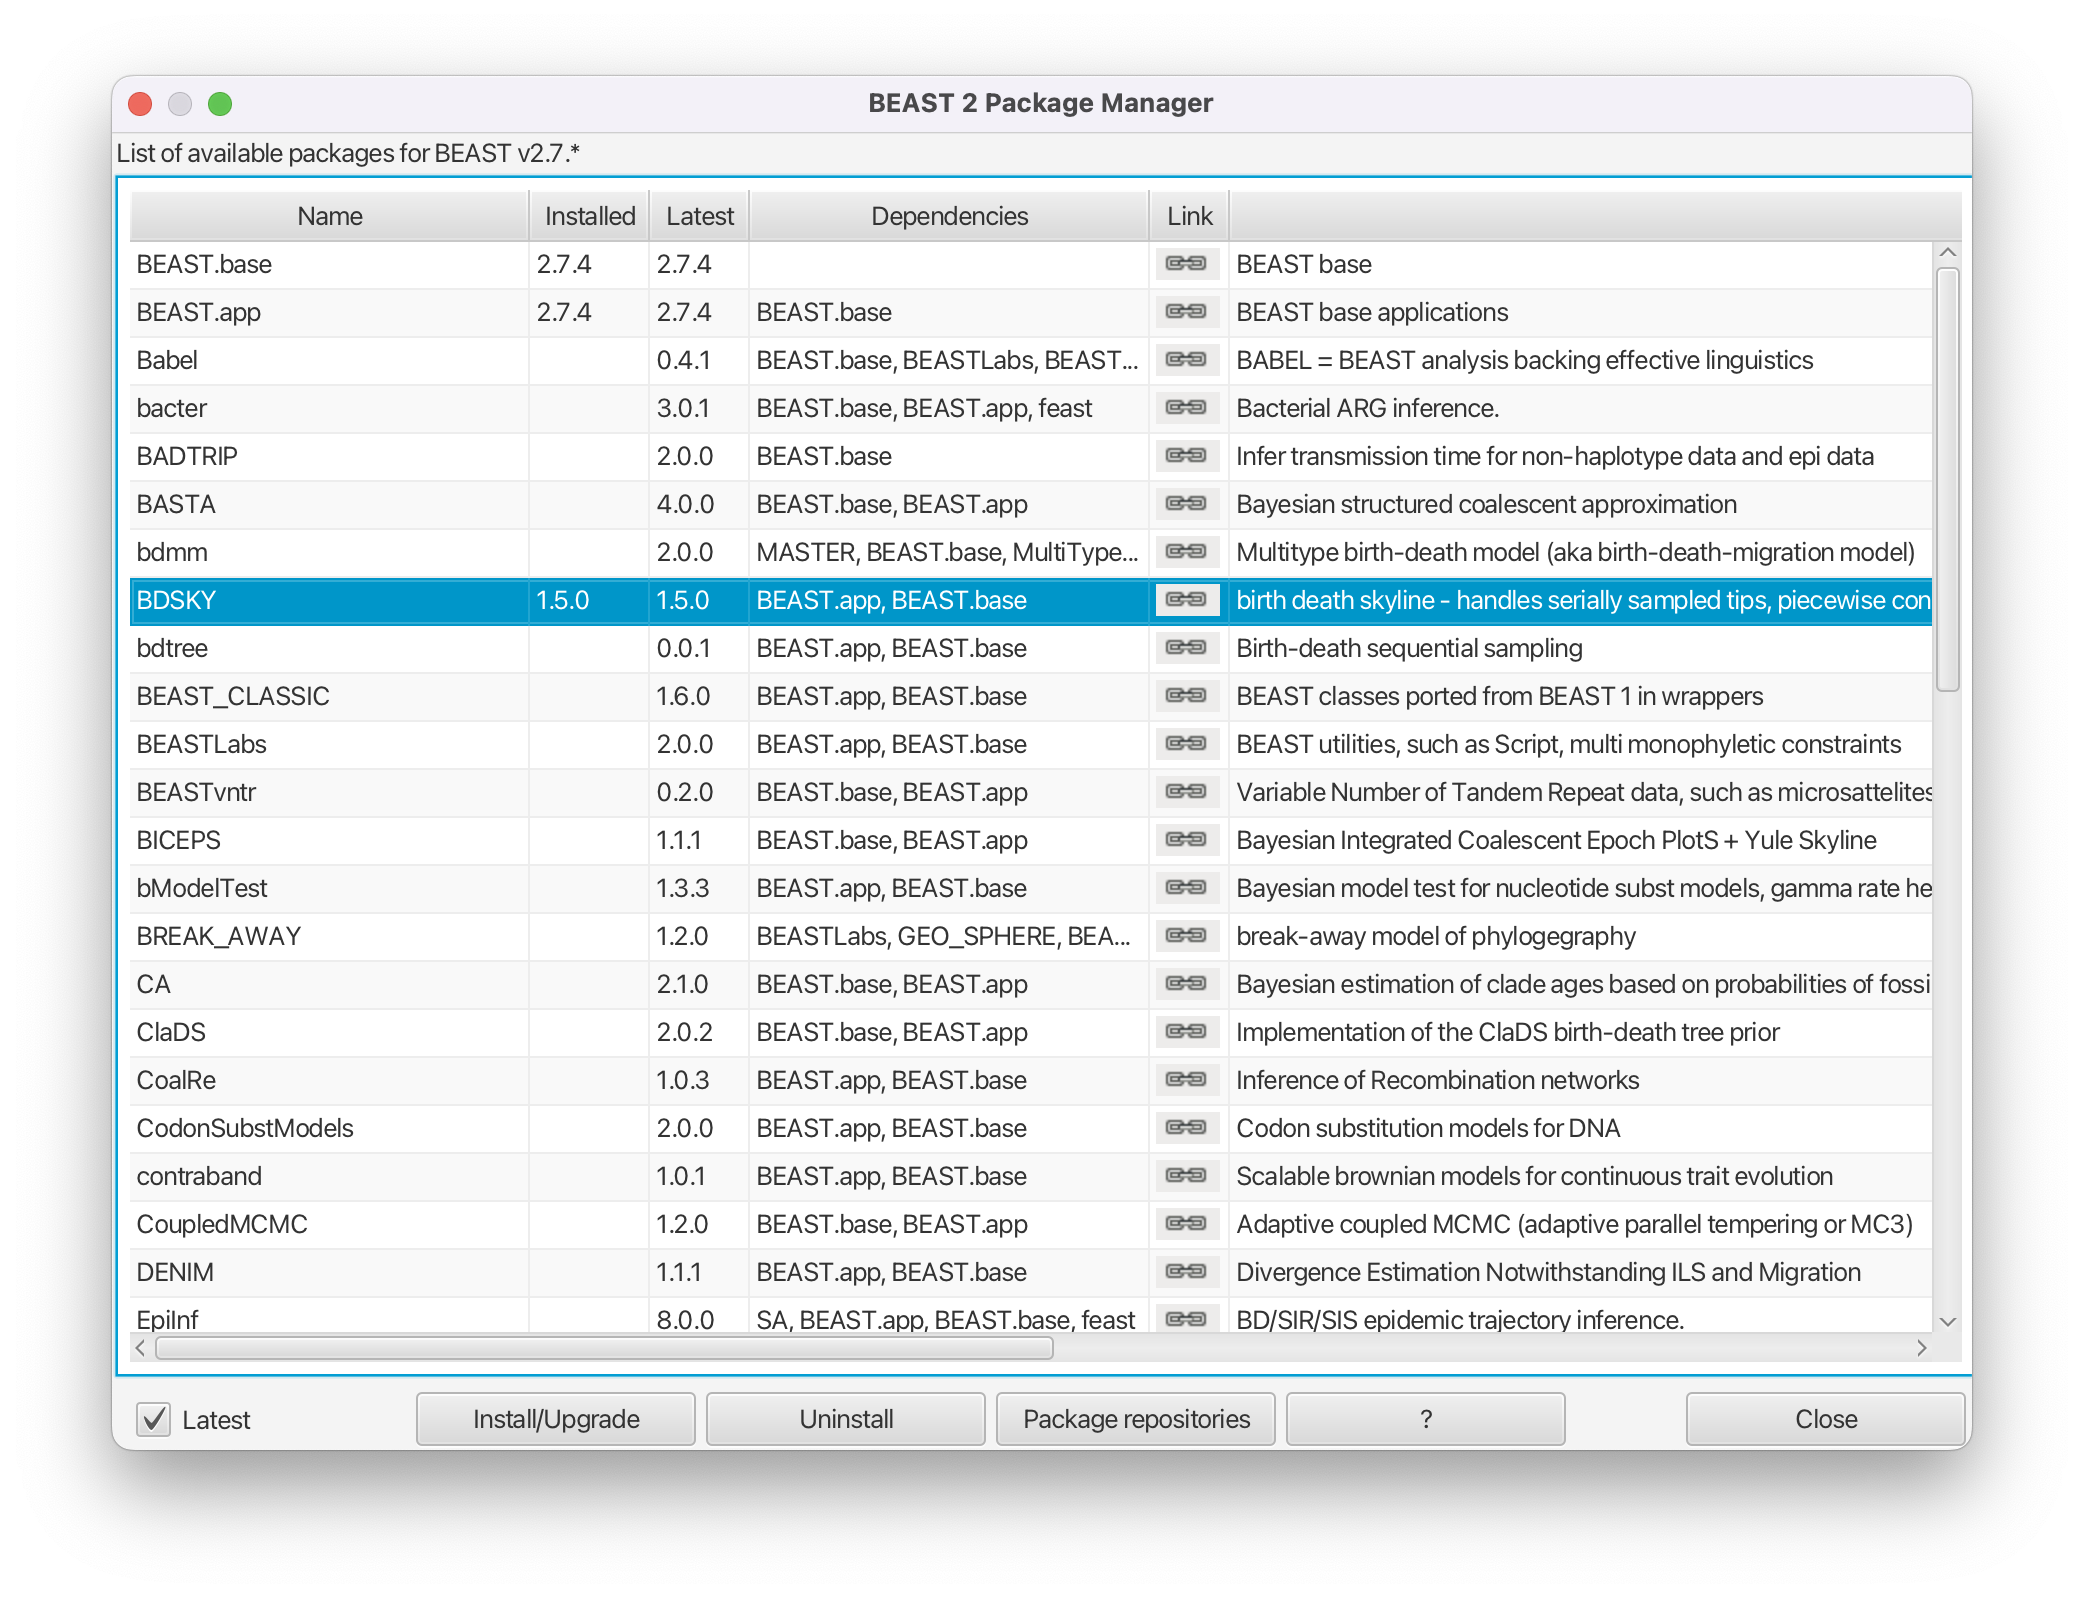
\includegraphics[width=0.750000\textwidth]{figures/install_bdsky.png}
    \caption{Install the BDSKY package which contains the Birth-Death Skyline model.}
    \label{fig:install}
\end{figure}

\clearpage

\hypertarget{setting-up-the-coalescent-bayesian-skyline-analysis}{%
\subsubsection{Setting up the Coalescent Bayesian Skyline
analysis}\label{setting-up-the-coalescent-bayesian-skyline-analysis}}

To start we have to import the alignment into BEAUti.

\begin{framed}
In the \textbf{Partitions} panel, import the nexus file with the
alignment by navigating to \textbf{File \textgreater{} Import Alignment}
in the menu and then finding the \passthrough{\lstinline!hcv.nexus!}
file on your computer \textbf{or} simply drag and drop the file into the
\textbf{BEAUti} window.
\end{framed}

BEAUti will recognize the sequences from the
\passthrough{\lstinline!*.nexus!} file as nucleotide data. It will do so
for sequence files with the character set of \textbf{A C G T N}, where
\textbf{N} indicates an unknown nucleotide. As soon as other non-gap
characters are included (e.g.~using \textbf{R} or \textbf{Y} to indicate
purines and pyramidines) BEAUti will not recognize the data as
nucleotides anymore (unless the type of data is specified in the
\passthrough{\lstinline!*.nexus!} file) and open a dialogue box to
confirm the data type.

The sequences were all sampled in 1993 so we are dealing with a
homochronous alignment and do not need to specify tip dates.

\begin{framed}
Skip the \textbf{Tip Dates} panel and navigate to the \textbf{Site
Model} panel.
\end{framed}

The next step is to specify the model of nucleotide evolution (the site
model). We will be using the GTR model, which is the most general
reversible model and estimates transition probabilities between
individual nucleotides separately. That means that the transition
probabilities between e.g.~\textbf{A} and \textbf{T} will be inferred
separately to the ones between \textbf{A} and \textbf{C}, however
transition probabilities from \textbf{A} to \textbf{C} will be the same
as \textbf{C} to \textbf{A} etc. (Note that the transition probabilities
here refer to the transition between \emph{any} two states in the
continuous time Markov-chain stochastic process that is used for the
substitution model, and not specifically to \emph{transitions} in the
context of genetics, i.e.~mutations from purines to purines or
pyramidines to pyramidines). Additionally, we allow for rate
heterogeneity among sites. We do this by changing the Gamma Category
Count to 4 (normally between 4 and 6).

\begin{framed}
Change the \textbf{Gamma Category Count} to 4, make sure that the
estimate box next to the \textbf{Shape} parameter of the Gamma
distribution is ticked and set \textbf{Subst Model} to \textbf{GTR}.
Make sure that the estimate box is ticked for all but one of the 6 rates
(there should be 5 ticked boxes) and that \textbf{Frequencies} are
estimated (Figure \ref{fig:model}).
\end{framed}

\begin{figure}
    \centering
    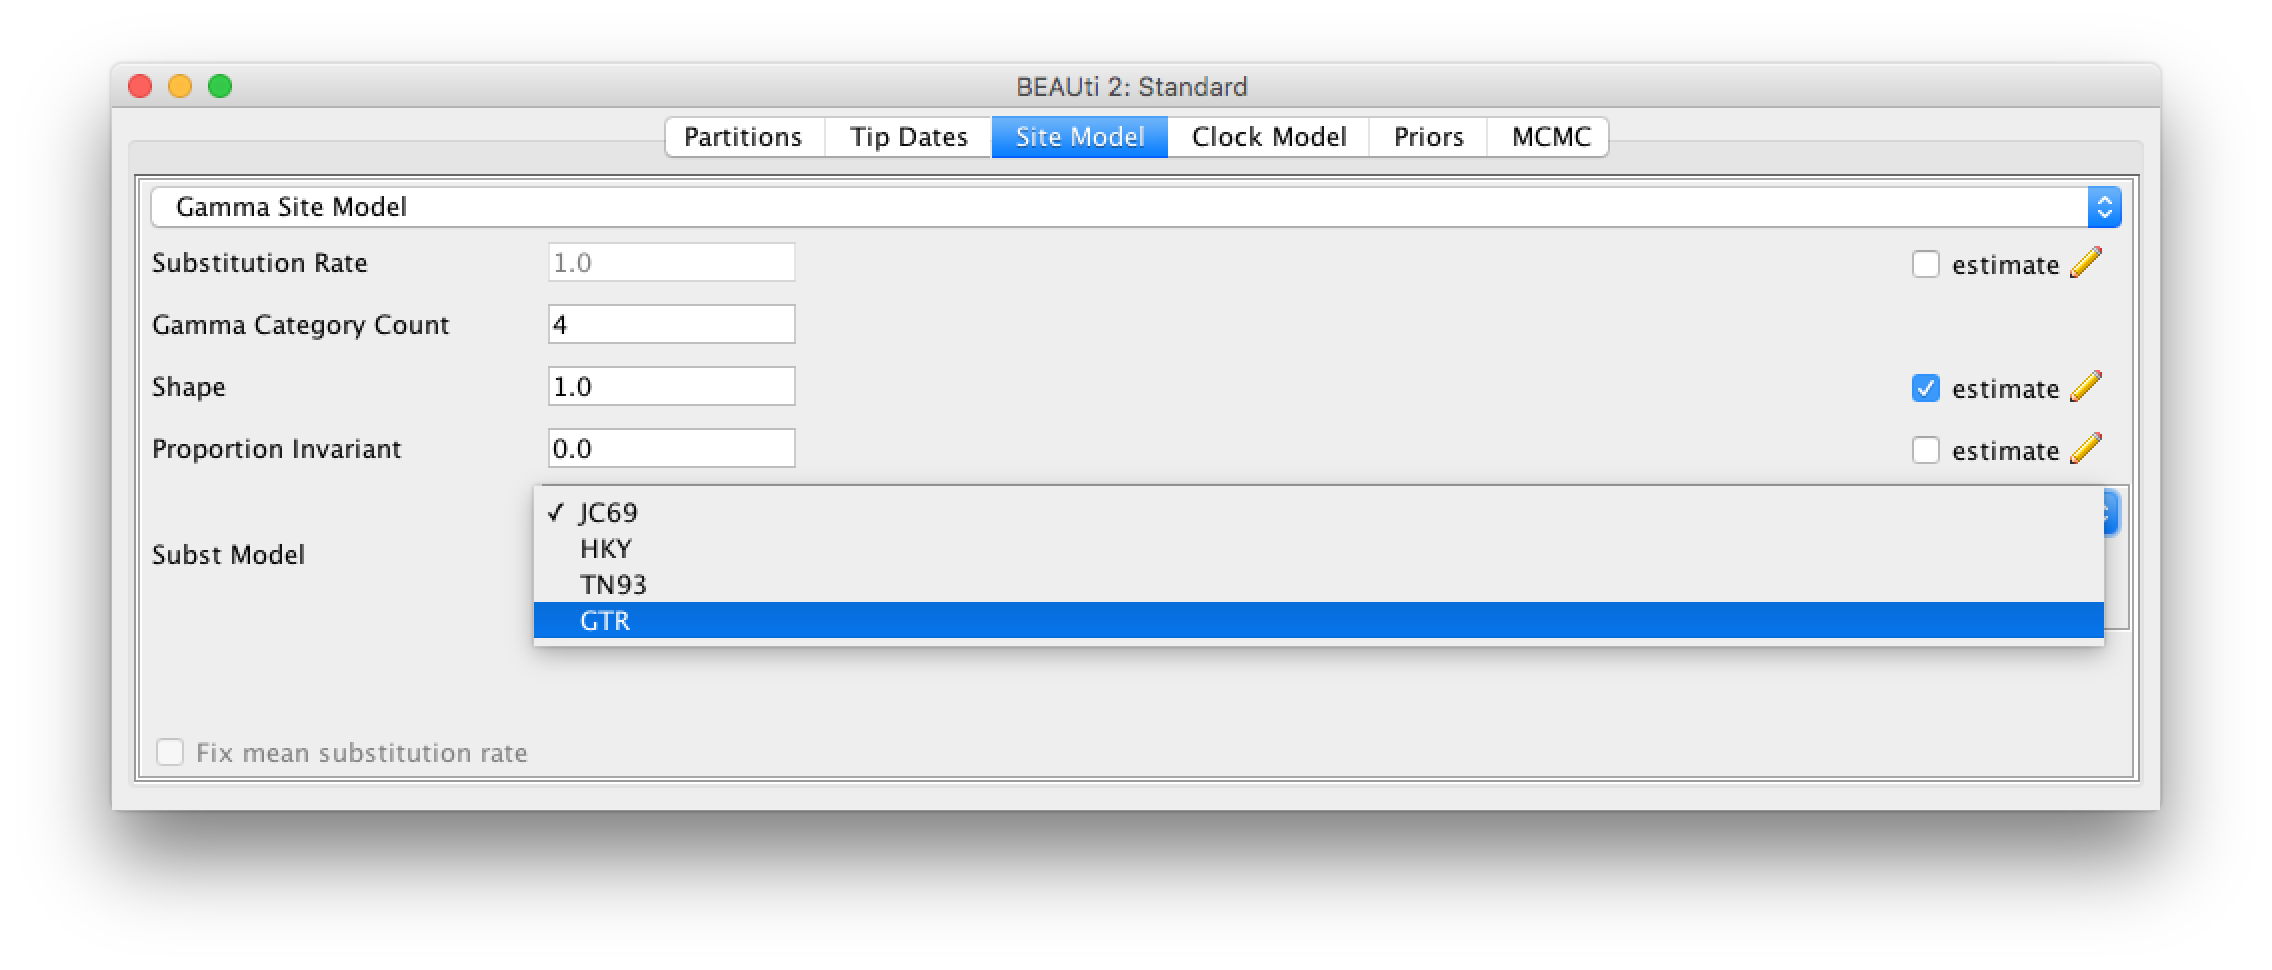
\includegraphics[max width=\textwidth, max height=0.9\textheight]{figures/choose_gtr.png}
    \caption{Set a GTR site model with a Gamma Category Count of 4.}
    \label{fig:model}
\end{figure}

\begin{framed}
\textbf{Topic for discussion:} Why are only 5 of the 6 rates of the GTR
model estimated?
\end{framed}

Because our sequences are contemporaneous (homochronous data) there is
no information in our dataset to estimate the clock rate (for more
information on this refer to the
\href{../Prior-selection/}{prior-selection} tutorial) and we have to use
external information to calibrate the clock. We will use an estimate
inferred in \citep{Pybus2001} to fix the clock rate. In this case all
the samples were contemporaneous (sampled at the same time) and the
clock rate is simply a scaling of the estimated tree branch lengths (in
substitutions/site) into calendar time.

\begin{framed}
Navigate to the \textbf{Clock Model} panel.

Leave the clock model as a \textbf{Strict Clock} and set
\textbf{Clock.rate} to 0.00079 s/s/y (Figure \ref{fig:clockmodel}).
(Note that BEAUti is smart enough to know that the clock rate cannot be
estimated on this dataset and grays out the estimate checkbox).
\end{framed}

\begin{figure}
    \centering
    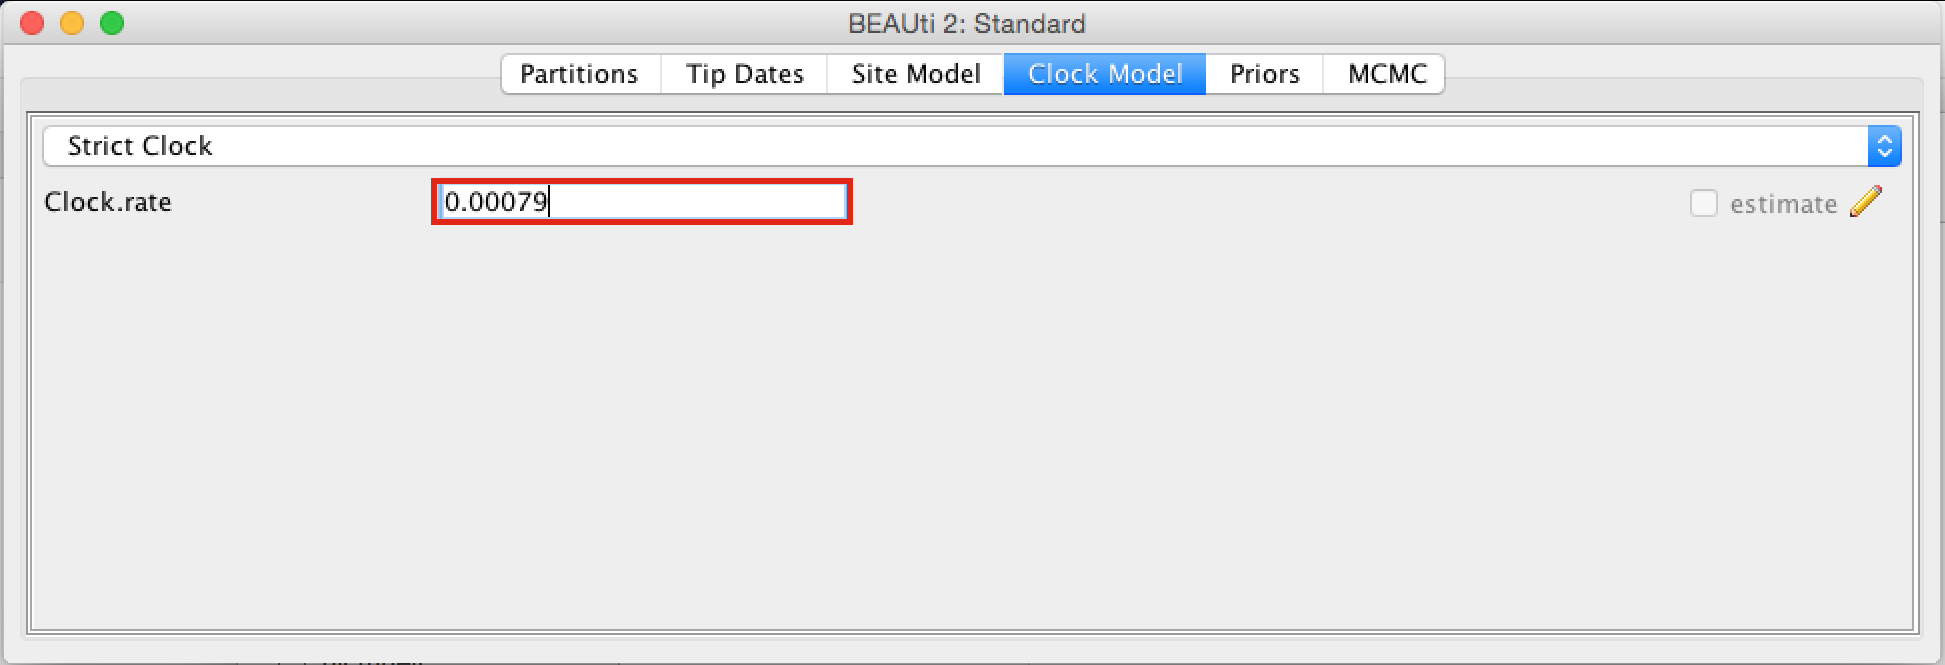
\includegraphics[max width=\textwidth, max height=0.9\textheight]{figures/set_clockrate.png}
    \caption{Set the clock rate to 0.00079 s/s/y.}
    \label{fig:clockmodel}
\end{figure}

Now we are ready to set up the Coalescent Bayesian Skyline as a
tree-prior.

\begin{framed}
Navigate to the \textbf{Priors} panel and select \textbf{Coalescent
Bayesian Skyline} as the tree prior (Figure \ref{fig:coalescent}).
\end{framed}

\begin{figure}
    \centering
    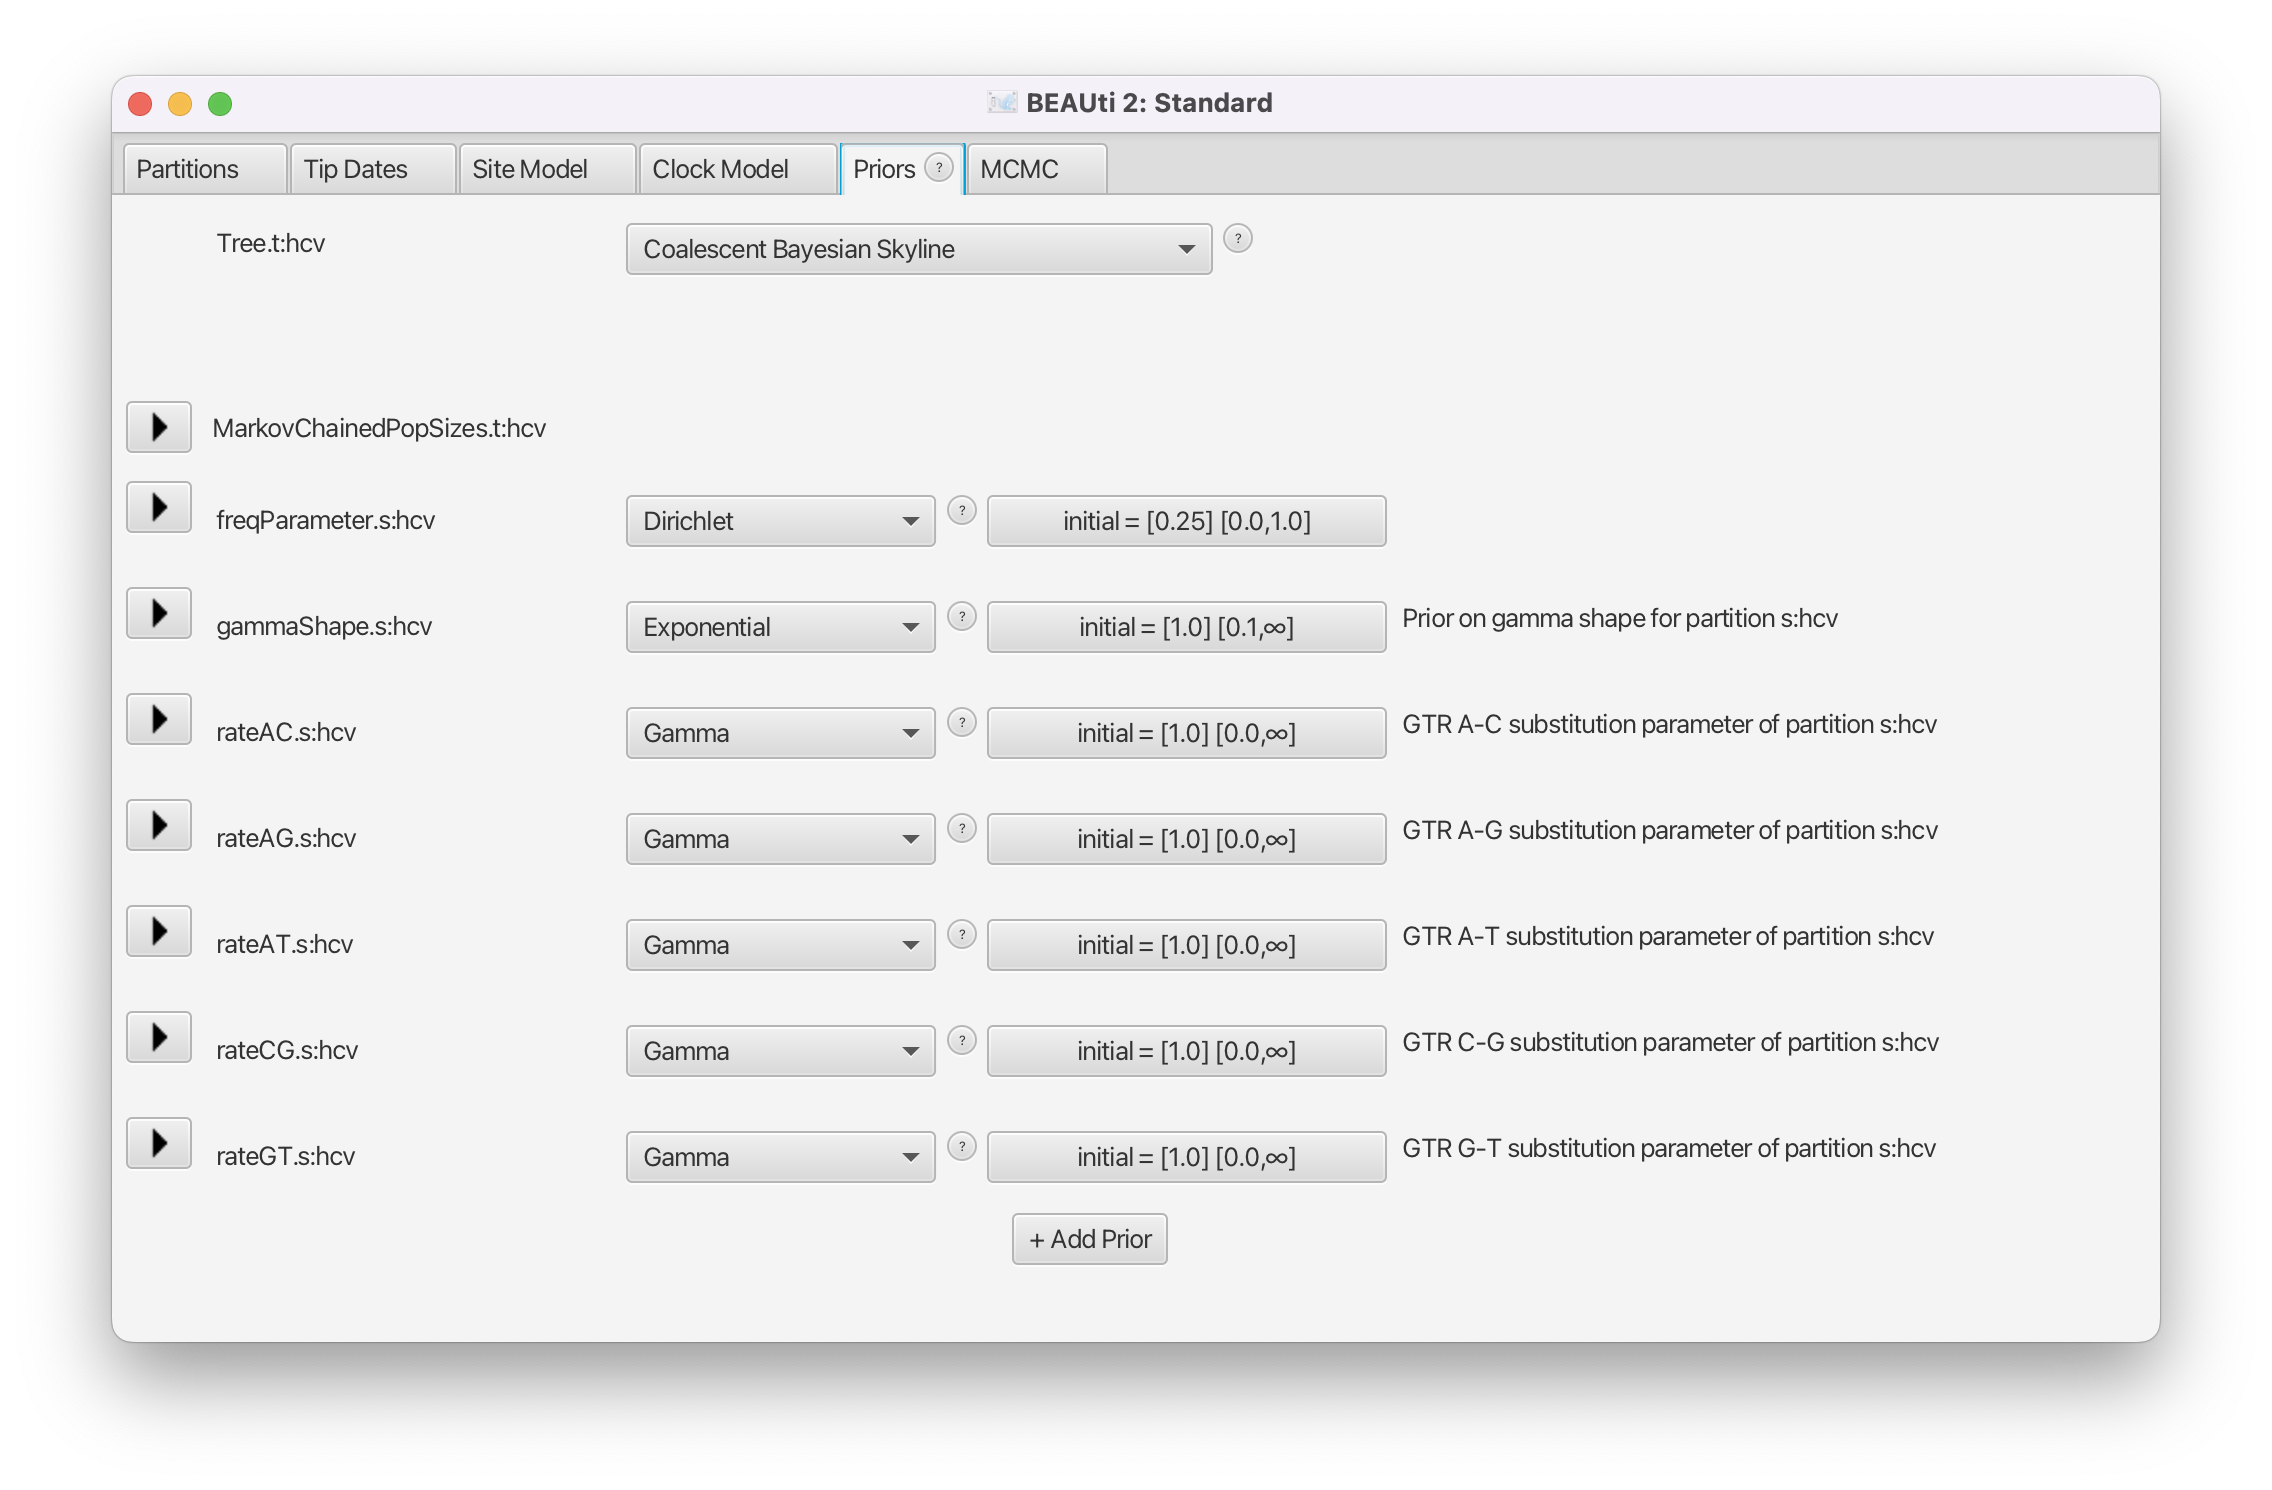
\includegraphics[max width=\textwidth, max height=0.9\textheight]{figures/choose_bsp.png}
    \caption{Choose the Coalescent Bayesian Skyline as a tree prior.}
    \label{fig:coalescent}
\end{figure}

The Coalescent Bayesian Skyline divides the time between the present and
the root of the tree (the tMRCA) into segments, and estimates a
different effective population size (\passthrough{$ N_e $})
for each segment. The endpoints of segments are tied to the branching
times (also called coalescent events) in the tree (Figure
\ref{fig:coal_events}), and the size of segments is measured in the
number of coalescent events included in each segment. The Coalescent
Bayesian Skyline groups coalescent events into segments and jointly
estimates the \passthrough{$ N_e $} (\textbf{bPopSizes}
parameter in BEAST) and the size of each segment (\textbf{bGroupSizes}
parameter). To set the number of segments we have to change the
dimension of \textbf{bPopSizes} and \textbf{bGroupSizes} (note that the
dimension of both parameters always has to be the same). Note that the
length of a segment is not fixed, but dependent on the timing of
coalescent events in the tree (Figure \ref{fig:coal_events}), as well as
the number of events contained within a segment (\textbf{bGroupSizes}).

\begin{figure}
    \centering
    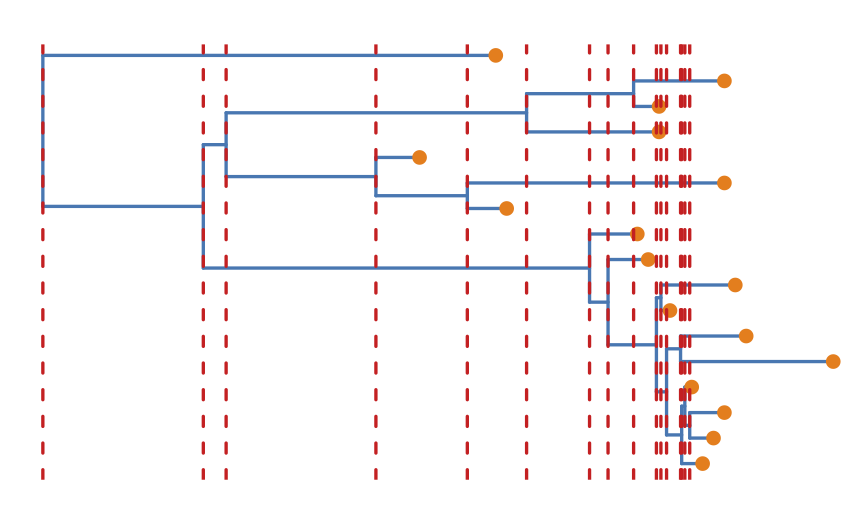
\includegraphics[width=0.750000\textwidth]{figures/coalescent_intervals.png}
    \caption{Example tree where the red dotted lines show the time-points of coalescent events.}
    \label{fig:coal_events}
\end{figure}

\begin{framed}
To change the number of segments we have to navigate to the
\textbf{Initialialization} panel, which is by default not visible.
Navigate to \textbf{View \textgreater{} Show Initialization Panel} to
make it visible and navigate to it (Figure \ref{fig:init}).

Set the dimension of \textbf{bPopSizes} and \textbf{bGroupSizes} to 4
(the default value is 5) after expanding the boxes for the two
parameters (Figure \ref{fig:dimensions}).
\end{framed}

\begin{figure}
    \centering
    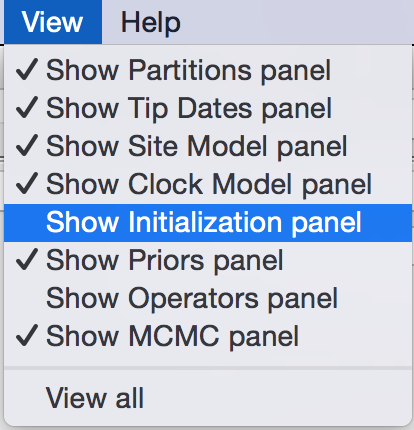
\includegraphics[width=0.250000\textwidth]{figures/goto_initialization.png}
    \caption{Show the initialization panel.}
    \label{fig:init}
\end{figure}

\begin{figure}
    \centering
    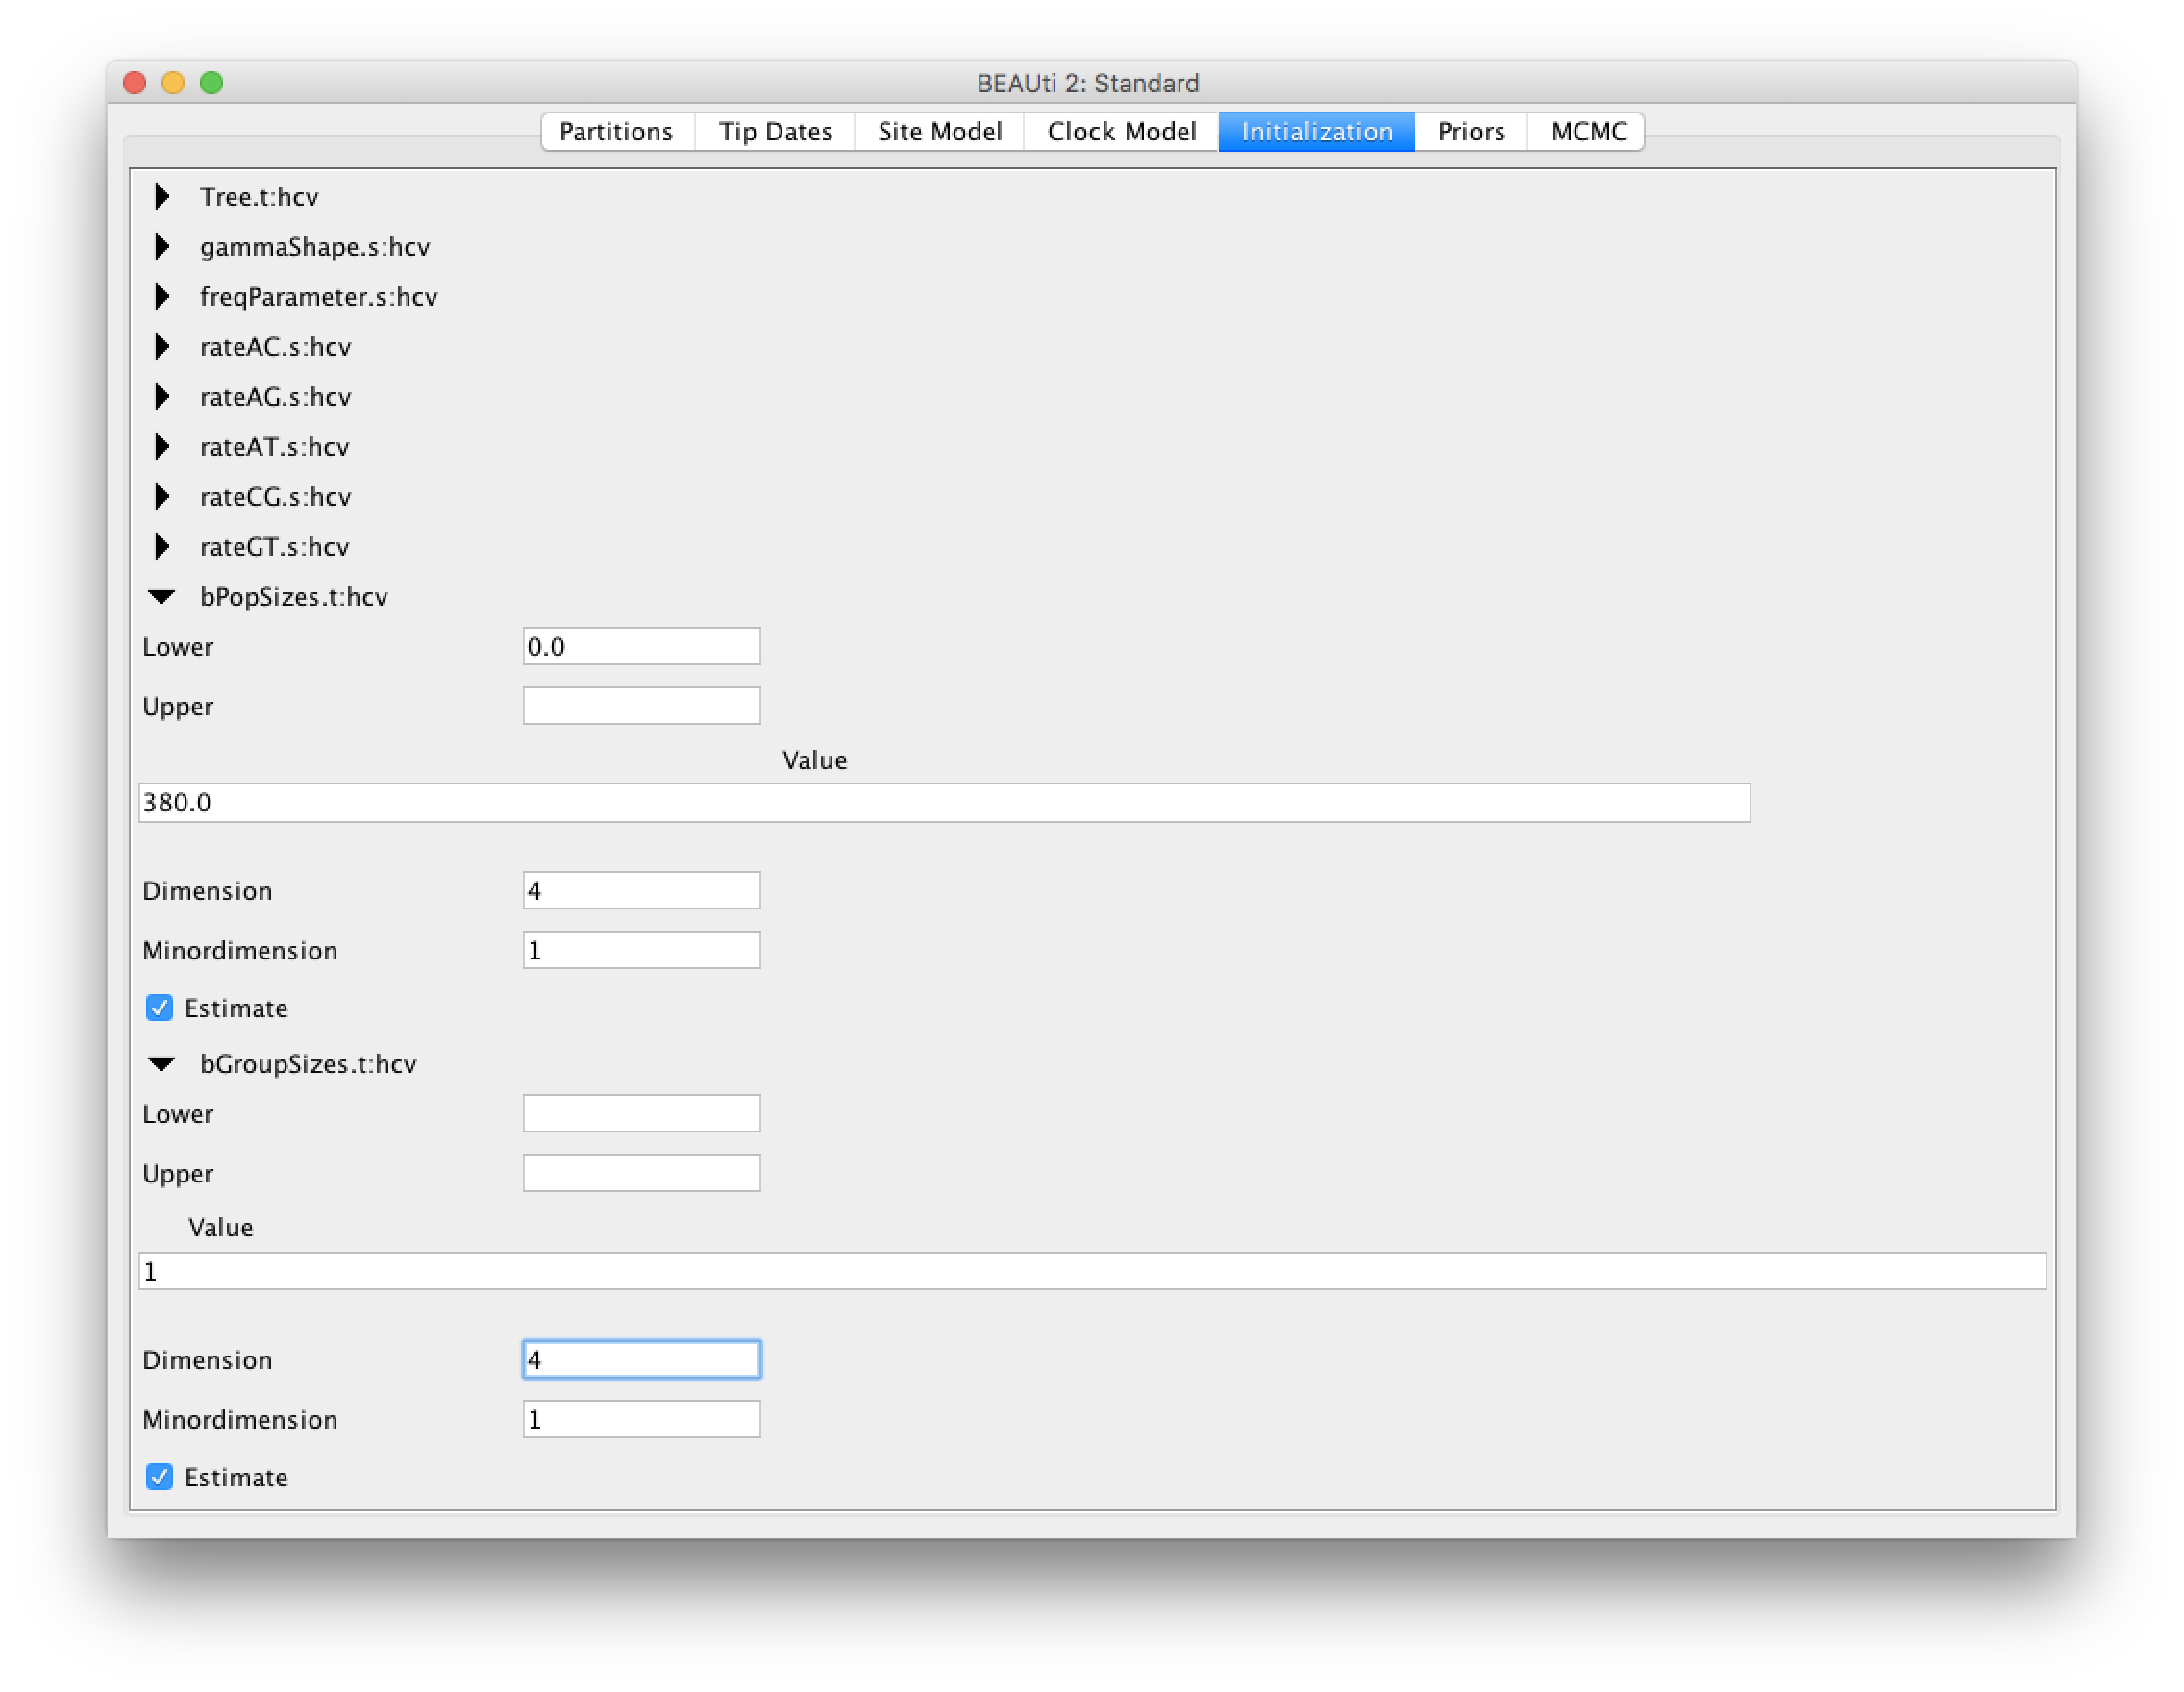
\includegraphics[max width=\textwidth, max height=0.9\textheight]{figures/set_dimension.png}
    \caption{Set the dimension of bPopSizes and bGroupSizes to 4.}
    \label{fig:dimensions}
\end{figure}

This sets the number of segments equal to 4 (the parameter dimension),
which means \passthrough{$ N_e $} will be allowed to change
3 times between the tMRCA and the present (if we have
\passthrough{$ d $} segments,
\passthrough{$ N_e $} is allowed to change
\passthrough{$ d-1 $} times).

We can leave the rest of the priors as they are and save the XML file.
We want to shorten the chain length and decrease the sampling frequency
so the analysis completes in a reasonable time and the output files stay
small. (Keep in mind that it will be necessary to run a longer chain for
parameters to mix properly).

\begin{framed}
Navigate to the \textbf{MCMC} panel.

Change the \textbf{Chain Length} from 10'000'000 to 3'000'000.

Click on the arrow next to the \textbf{tracelog} and change the
\textbf{File Name} to \passthrough{\lstinline!\$(filebase).log!} and set
the \textbf{Log Every} to 3'000.

Click on the arrow next to the \textbf{treelog} and change the
\textbf{File Name} to \passthrough{\lstinline!\$(filebase)-\$(tree).log!}
and set the \textbf{Log Every} to 3'000.

Leave all other settings at their default values and save the file as
\passthrough{\lstinline!hcv_coal.xml!}.

(Note that since BEAST 2.7 the filenames used here are the default
filenames and should not need to be changed!)
\end{framed}

When we run the analysis \passthrough{lstinline!\$(filebase)!} in the
name of the \passthrough{\lstinline!*.log!} and
\passthrough{\lstinline!*.trees!} files will be replaced by the name of
the XML file. This is a good idea, since it makes it easy to keep track
of which XML files produced which output files.

Now we are ready to run the analysis.

\begin{framed}
Start \textbf{BEAST2} and choose the file
\passthrough{\lstinline!hcv_coal.xml!}.

If you have \textbf{BEAGLE} installed tick the box to \textbf{Use BEAGLE
library if available}, which will make the analysis run faster.

Hit \textbf{Run} to start the analysis.
\end{framed}

The analysis will take about 10 minutes to complete. Read through the
next section while waiting for your results or start preparing the XML
file for the \protect\hyperlink{sec:bdsky}{birth-death skyline}
analysis.

\hypertarget{the-coalescent-bayesian-skyline-parameterization}{%
\subsubsection{The Coalescent Bayesian Skyline
parameterization}\label{the-coalescent-bayesian-skyline-parameterization}}

The Coalescent Bayesian Skyline model uses the Kingman coalescent for
each segment, which assumes that the sequences are a small sample drawn
from a haploid population evolving under Wright-Fisher dynamics (Figure
\ref{fig:wrightfisher}). The model works by calculating the probability
of observing the tree under this assumption. This essentially boils down
to repeatedly asking the question of how likely it is for two lineages
to coalesce (have a common ancestor) in a given time.

\begin{figure}
    \centering
    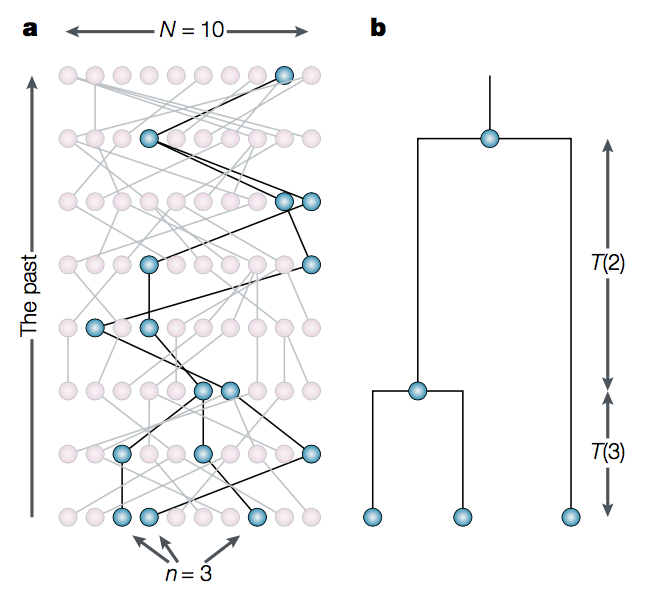
\includegraphics[width=0.500000\textwidth]{figures/Rosenberg2002.png}
    \caption{The basic principle behind the coalescent. Figure from \citep{Rosenberg2002}.}
    \label{fig:wrightfisher}
\end{figure}

The effective population size (\passthrough{$ N_e $}) is
the inverse of the rate of coalescence
\passthrough{$ \lambda $}. The larger
\passthrough{$ N_e $} is the less likely lineages are to
coalesce. Thus, intervals in a sampled tree with many branching events
often coincide with periods when the population size was small.
Similarly, few branching events occur during periods of large population
size. (Note that these results are conditioned on sampling only a small
fraction of the population).

\begin{equation}
    \lambda = \frac{1}{N_e}
\end{equation}

For an SIR model (\textbf{S}usceptible, \textbf{I}nfected and
\textbf{R}ecovered), \passthrough{$ N_e $} is proportional
to the overall population size \passthrough{$ N $} and the
number of infected \passthrough{$ I $} and inversely
proportional to the transmission rate
\passthrough{$ \theta $}.

\begin{equation}
    N_e = \frac{I}{\theta} \frac{N}{S}
\end{equation}

Estimates of \passthrough{$ N_e $} therefore do not
directly tell us something about the number of infected, nor the
transmission rate. However, changes in
\passthrough{$ N_e $} can be informative about changes in
the transmission rate or the number of infected (if they do not cancel
out).

The Coalescent Bayesian Skyline model allows
\passthrough{$ N_e $} to change over time in a
nonparametric fashion (i.e.~we do not have to specify an equation
governing changes in \passthrough{$ N_e $} over time).
Another way to think about the model is as maximally-parameterized,
since it infers \passthrough{$ d $} change-point times
(segment boundaries) and a value for \passthrough{$ N_e $}
in each segment. This makes the Bayesian Skyline flexible enough to
model very complicated \passthrough{$ N_e $} dynamics,
provided that enough segments are specified. It may be tempting to
specify the maximum dimension for the model (each group contains only
one coalescent event, thus \passthrough{$ N_e $} changes at
each branching time in the tree), making it as flexible as possible.
This is the parameterization used by the Classic Skyline plot
\citep{Pybus2000}, which is the direct ancestor of the Coalescent
Bayesian Skyline plot. However, the only informative events used by the
Coalescent Bayesian Skyline plot are the coalescent events. Thus, using
a maximally-flexible parameterization with only one informative event
per segment often leads to erratic and noisy estimates of
\passthrough{$ N_e $} over time (especially if segments are
very short, see Figure \ref{fig:coal_events}). Grouping segments
together leads to smoother and more robust estimates.

Choosing the dimension for the Bayesian Skyline can be rather arbitrary.
If the dimension is chosen too low, not all population size changes are
captured, but if it is chosen too large, there may be too little
information in a segment to support a robust estimate. When trying to
decide if the dimension is appropriate it may be useful to consider the
average number of informative (coalescent) events per segment. (A tree
of \passthrough{$ n $} taxa has
\passthrough{$ n-1 $} coalescences, thus
\passthrough{$ N_e $} in each segment is estimated from on
average \passthrough{$ \frac\{n-1\}\{d\} $} informative
data points). Would this number of random samples drawn from a
hypothetical distribution allow you to accurately estimate the
distribution? If not, consider decreasing the dimension. There are
descendants of the coalescent skyline in BEAST that either estimate the
number of segments (Extended Bayesian Skyline \citep{Heled2008}) or do
not require the number of segments to be specified (Skyride
\citep{Minin2008}), but instead makes very strong prior assumptions
about changes in \passthrough{$ N_e $}.

\hypertarget{exploring-the-results-of-the-coalescent-bayesian-skyline-analysis}{%
\subsubsection{Exploring the results of the Coalescent Bayesian Skyline
analysis}\label{exploring-the-results-of-the-coalescent-bayesian-skyline-analysis}}

For the reconstruction of the population dynamics, we need two files,
the \passthrough{\lstinline!*.log!} file and the
\passthrough{\lstinline!*.trees!} file. The log file contains the
information about the group sizes and population sizes of each segment,
while the trees file is needed for the times of the coalescent events.

\begin{framed}
Load the logfile into \textbf{Tracer} to check mixing and parameter
estimates (Figure \ref{fig:tracer_bsp}).
\end{framed}

\begin{figure}
    \centering
    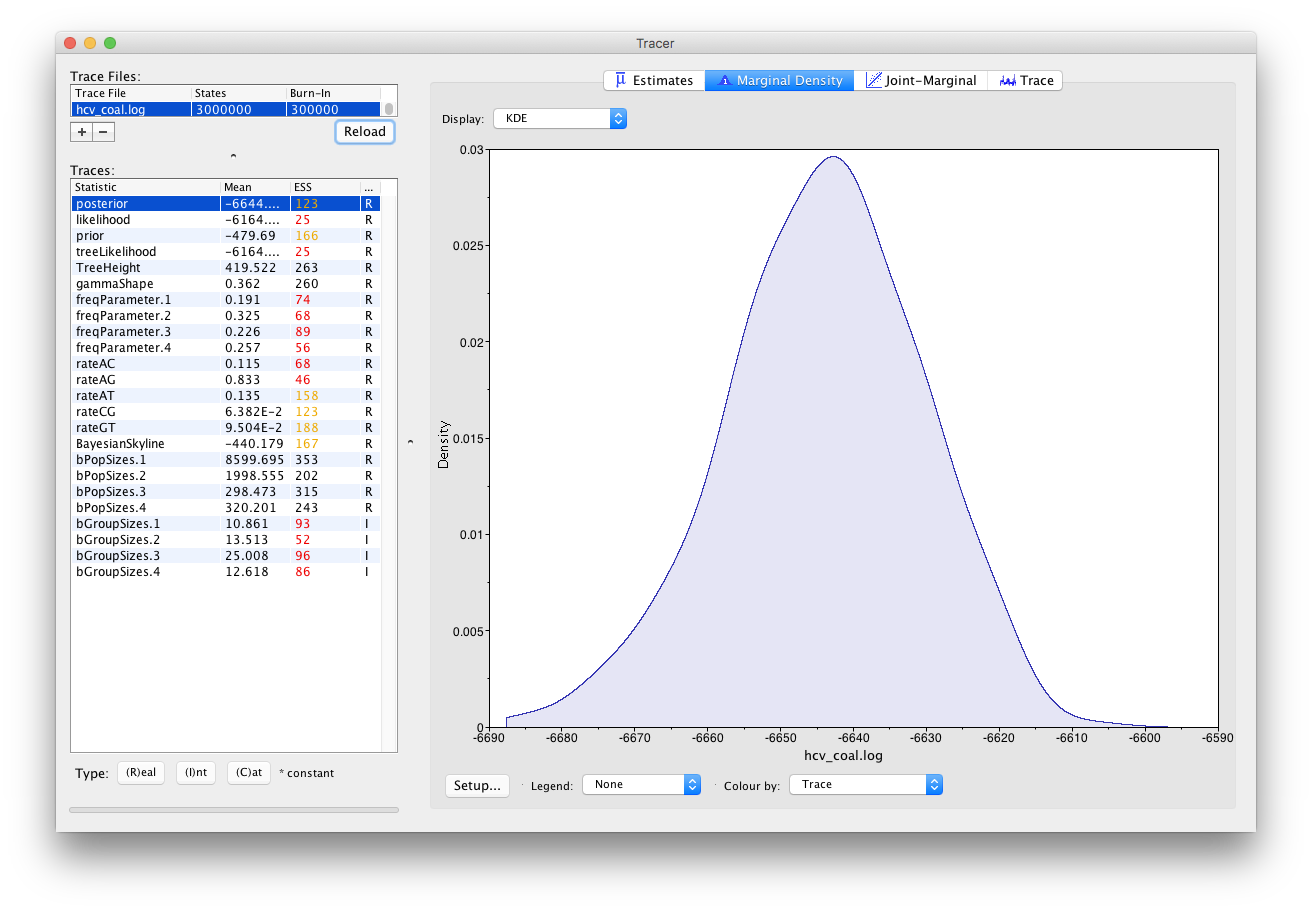
\includegraphics[max width=\textwidth, max height=0.9\textheight]{figures/bsp_tracer.png}
    \caption{Loading the log file into Tracer.}
    \label{fig:tracer_bsp}
\end{figure}

Because we shortened the chain most parameters have very low ESS values.
If you like, you can compare your results with the example results we
obtained with identical settings and a chain of 30,000,000
(\passthrough{\lstinline!hcv_coal_30M.log!}).

\begin{framed}
Navigate to \textbf{Analysis \textgreater{} Bayesian Skyline
Reconstruction}. From there open the \passthrough{\lstinline!*.trees!}
file. To get the correct dates in the analysis we should specify the
\textbf{Age of the youngest tip}. In our case it is 1993, the year where
all the samples were taken. If the sequences were sampled at different
times (heterochronous data), the age of the youngest tip is the time
when the most recent sample was collected.

Press \textbf{OK} to reconstruct the past population dynamics (Figure
\ref{fig:trees}).
\end{framed}

\begin{figure}
    \centering
    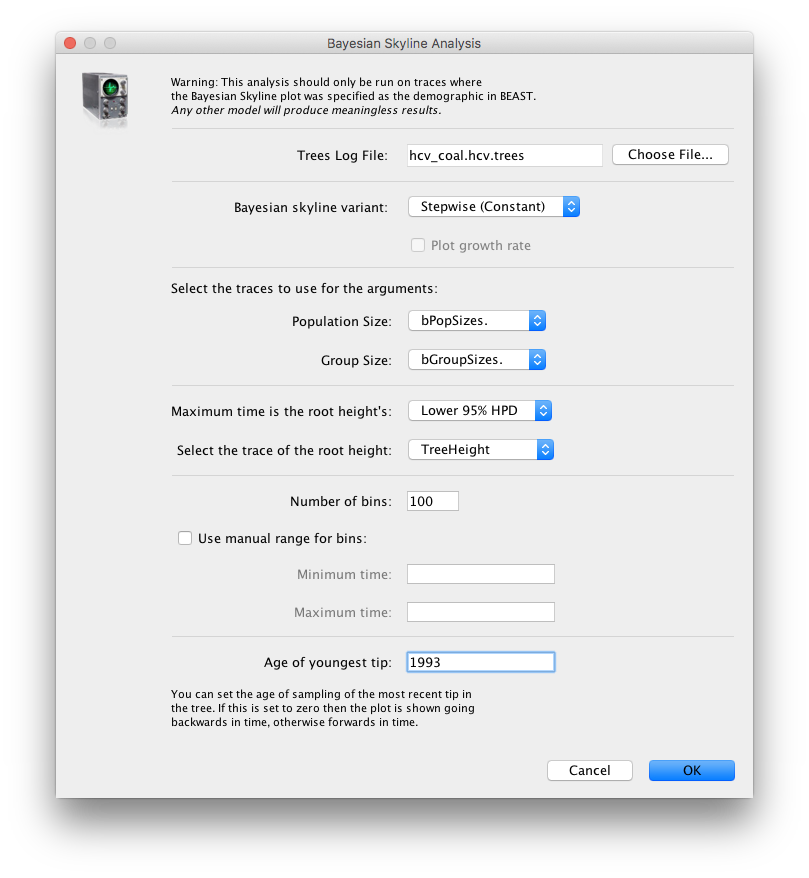
\includegraphics[width=0.750000\textwidth]{figures/open_trees.png}
    \caption{Reconstructing the Bayesian Skyline plot in Tracer.}
    \label{fig:trees}
\end{figure}

The output will have the years on the x-axis and the effective
population size on the y-axis. By default, the y-axis is on a log-scale.
If everything worked as it is supposed to work you will see a sharp
increase in the effective population size in the mid 20th century,
similar to what is seen on Figure \ref{fig:skyline}.

(Note that the reconstruction will only work if the
\passthrough{\lstinline!*.log!} and \passthrough{\lstinline!*.trees!}
files contain the exact same number of states and both files were logged
at the same frequency).

\begin{figure}
    \centering
    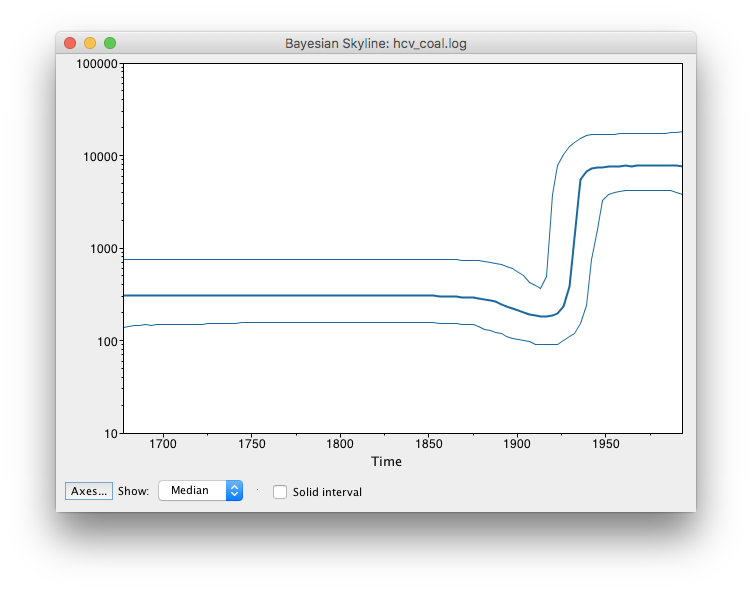
\includegraphics[width=0.750000\textwidth]{figures/skyline_analysis.png}
    \caption{Coalescent Bayesian Skyline analysis output. The black line is the median estimate of the estimated effective population size (can be changed to the mean estimate). The two blue lines are the upper and lower bounds of the 95\% HPD interval. The x-axis is the time in years and the y-axis is on a log-scale.}
    \label{fig:skyline}
\end{figure}

There are two ways to save the analysis, it can either be saved as a
\passthrough{\lstinline!*.pdf!} for display purposes or as a tab
delimited file.

\begin{framed}
Navigate to \textbf{File \textgreater{} Export Data Table}.

Enter the filename as \passthrough{\lstinline!hcv_coal.tsv!} and save
the file.
\end{framed}

The exported file will have five rows, the time, the mean, median, lower
and upper boundary of the 95\% HPD interval of the estimates, which you
can use to plot the data with other software (R, Matlab, etc).

\hypertarget{choosing-the-dimension}{%
\subsubsection{Choosing the Dimension}\label{choosing-the-dimension}}

If we compare the estimates of the population dynamics using different
dimensions, we see that most of the dynamics are already captured with
having only 2 dimensions, as shown in Figure \ref{fig:comparison}.
Adding more dimensions only changes the inferred effective population
size before 1900. Note that adding more dimensions adds a slight dip
before the increase in the effective population size (around 1900). When
comparing to the HPD intervals (Figure \ref{fig:skyline}) we see that
this dip is not significant and may not be indicative of a real decrease
in the effective population size before the subsequent increase.

\begin{figure}
    \centering
    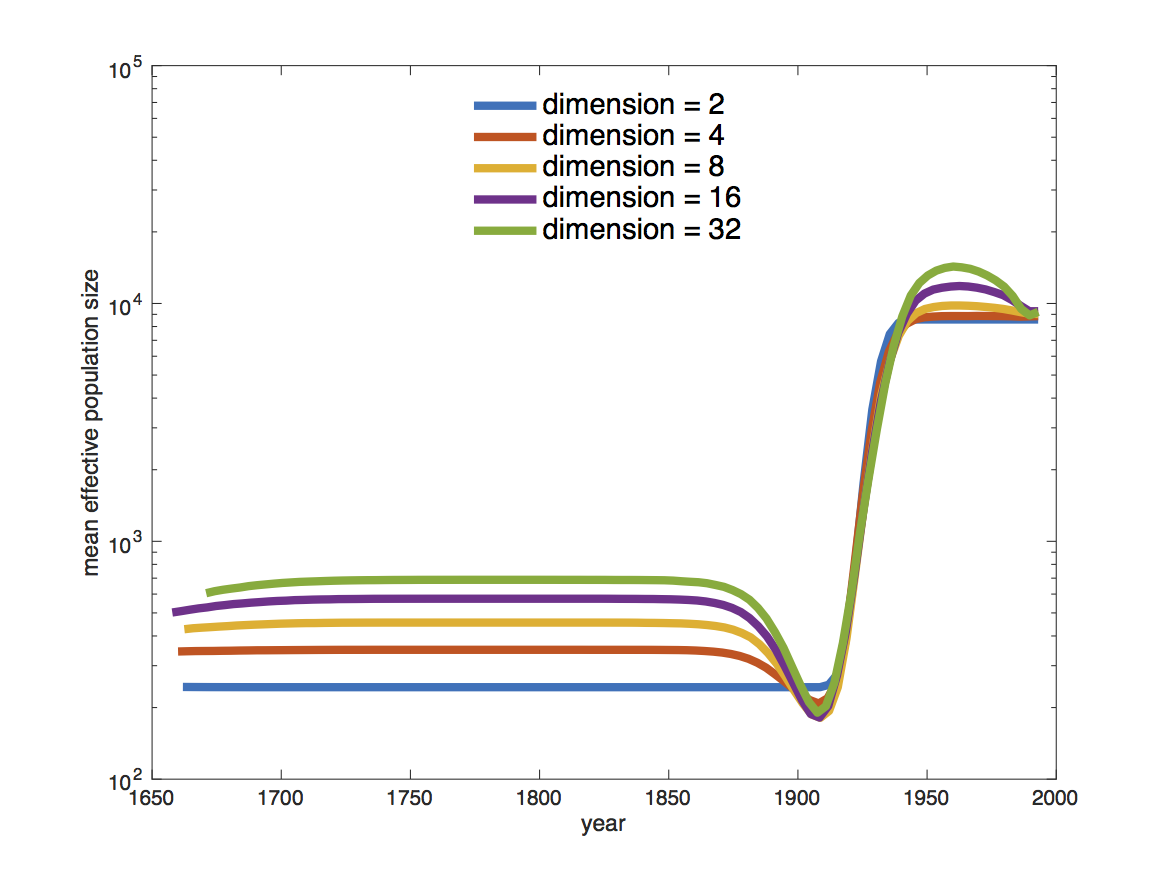
\includegraphics[width=1.000000\textwidth]{figures/comparison_dimension.png}
    \caption{Estimated mean effective population sizes using different dimensions.}
    \label{fig:comparison}
\end{figure}

The choice of the number of dimensions can also have a direct effect on
how fast the MCMC converges (Figure \ref{fig:ess}). The slower
convergence with increasing dimension can be caused by e.g.~less
information per interval. To some extent it is simply caused by the need
to estimate more parameters though.

\begin{figure}
    \centering
    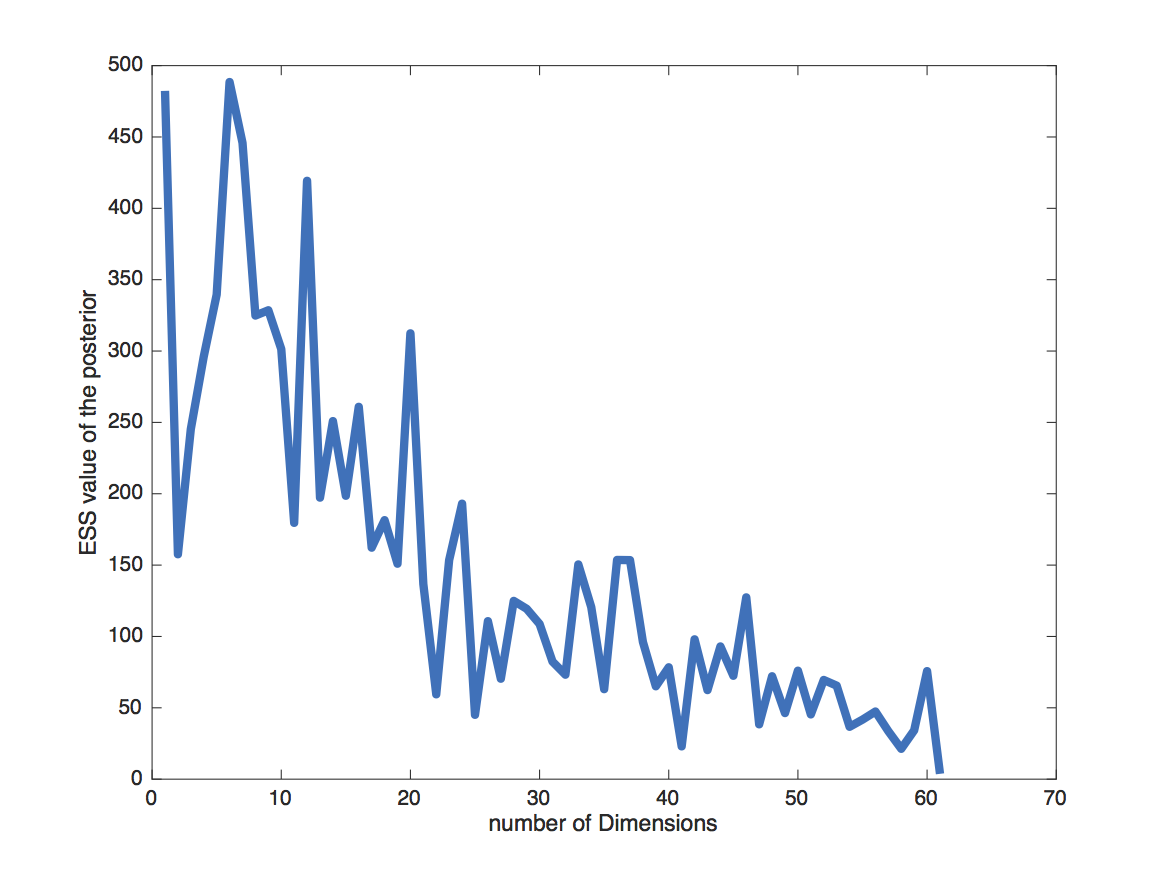
\includegraphics[width=0.500000\textwidth]{figures/ess_vs_dim_coal.png}
    \caption{The ESS value of the posterior after running an MCMC chain with `$ 10^7 $` samples, logged every `$ 10^3 $` steps and a burnin of 10\% for using different dimensions of the Coalescent Bayesian Skyline.}
    \label{fig:ess}
\end{figure}

\clearpage

\hypertarget{setting-up-the-birth-death-skyline-analysis}{%
\subsubsection{Setting up the Birth-Death Skyline
analysis}\label{setting-up-the-birth-death-skyline-analysis}}

In the first analysis, we used the coalescent approach to estimate
population dynamics. We now want to repeat the analysis using the
Birth-Death Skyline model. We will use the same model setup as in the
previous analysis and only change the tree prior.

\begin{framed}
Restart \textbf{BEAUti}, load \passthrough{\lstinline!hcv.nexus!} as
before and set up the same site and clock model as in the Coalescent
Bayesian Skyline analysis.
\end{framed}

We will need to set the prior to \textbf{Birth Death Skyline
Contemporary}, since the sequences were all sampled at the same point in
time. For heterochronous data (sequences sampled at different times), we
would use \textbf{Birth Death Skyline Serial}. As with the Coalescent
Bayesian Skyline, we need to set the number of dimensions. Here we set
the dimension for \passthrough{$ R_e $}, the effective
reproduction number, which denotes the average number of secondary
infections caused by an infected person at a given time during the
epidemic, i.e.~an \passthrough{$ R_e $} of 2 would mean
that every infected person causes two new infections on average. In
other words, an \passthrough{$ R_e $} above 1 means that
the number of cases are increasing, therefore the disease will cause an
exponentially growing epidemic, and an
\passthrough{$ R_e $} below 1 means that the epidemic will
die out.

\begin{framed}
Navigate to the \textbf{Priors} panel and select \textbf{Birth Death
Skyline Contemporary} as the tree prior (Figure \ref{fig:bdsky}).

Then, click on the button where it says \textbf{initial = {[}2.0{]}
{[}0.0, Infinity{]}} next to \textbf{reproductiveNumber}. A pop-up
window will open which allows us to change the dimension of the
parameter (Figure \ref{fig:dimensions_bdsky}). In this case we will keep
the default dimension of 10.

Press \textbf{OK} to close the pop-up window.
\end{framed}

\begin{figure}
    \centering
    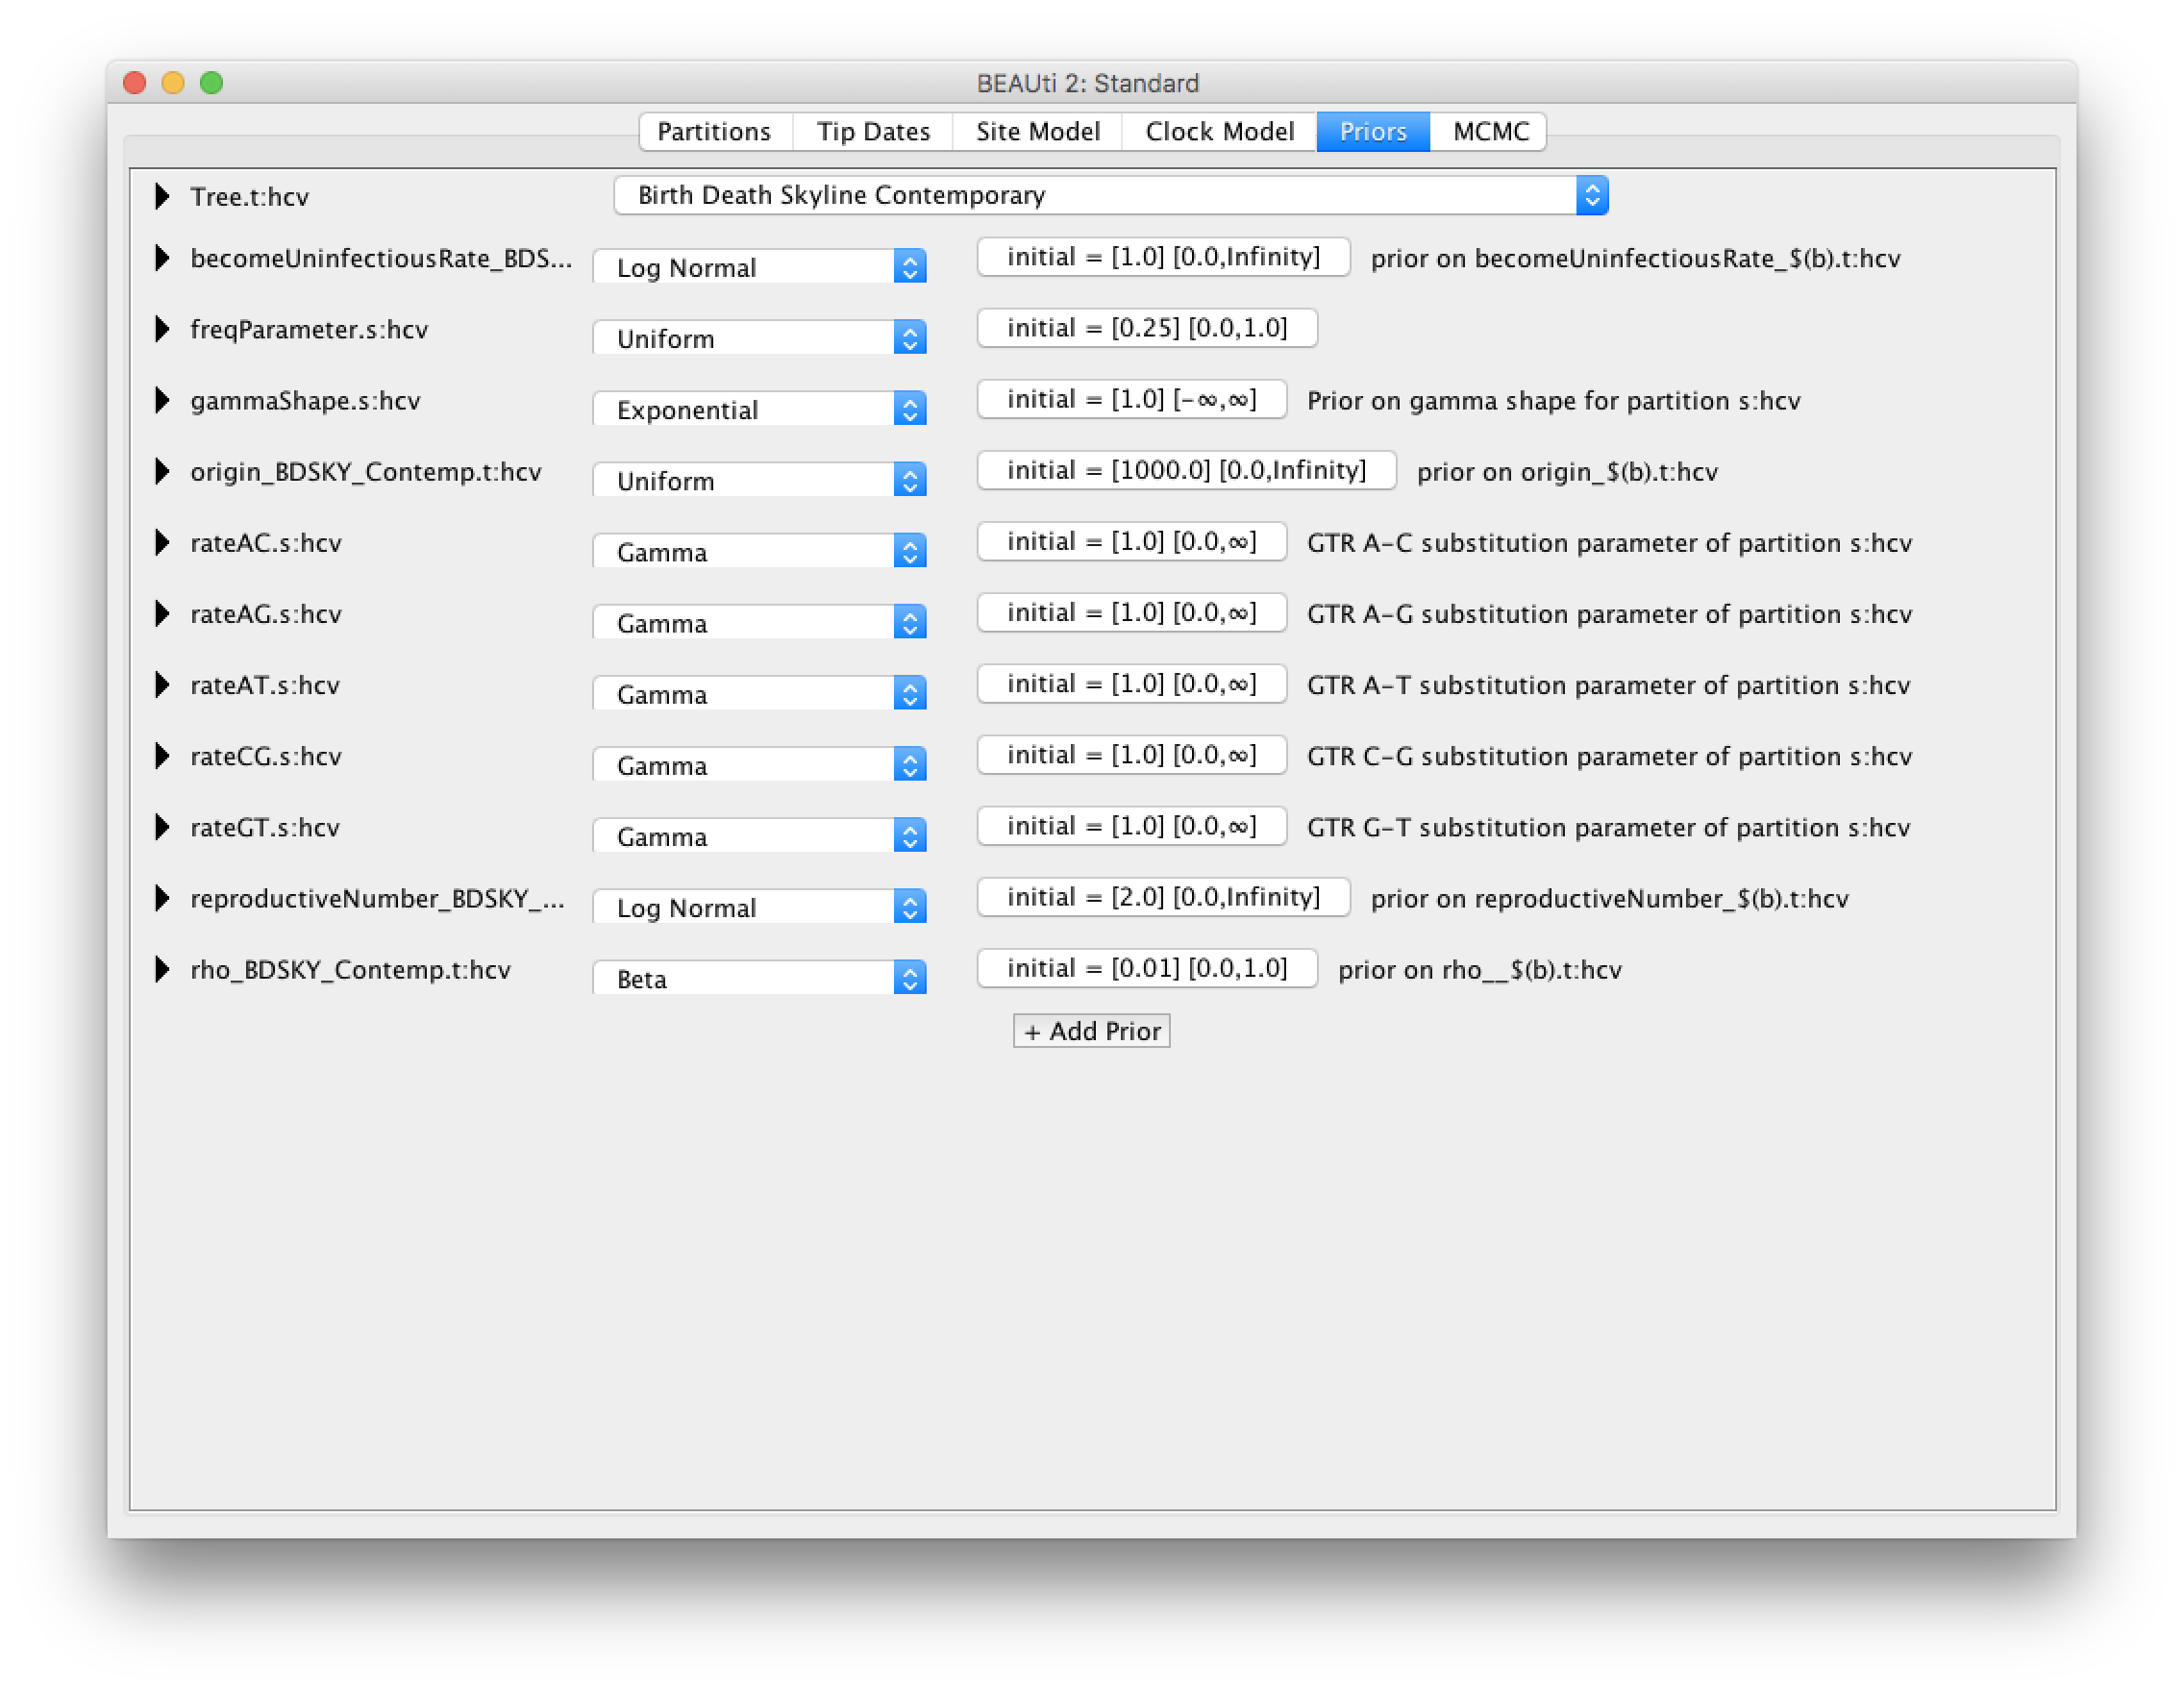
\includegraphics[max width=\textwidth, max height=0.9\textheight]{figures/choose_bdsky.png}
    \caption{Setting the prior on the tree to the Birth-Death Skyline.}
    \label{fig:bdsky}
\end{figure}

\begin{figure}
    \centering
    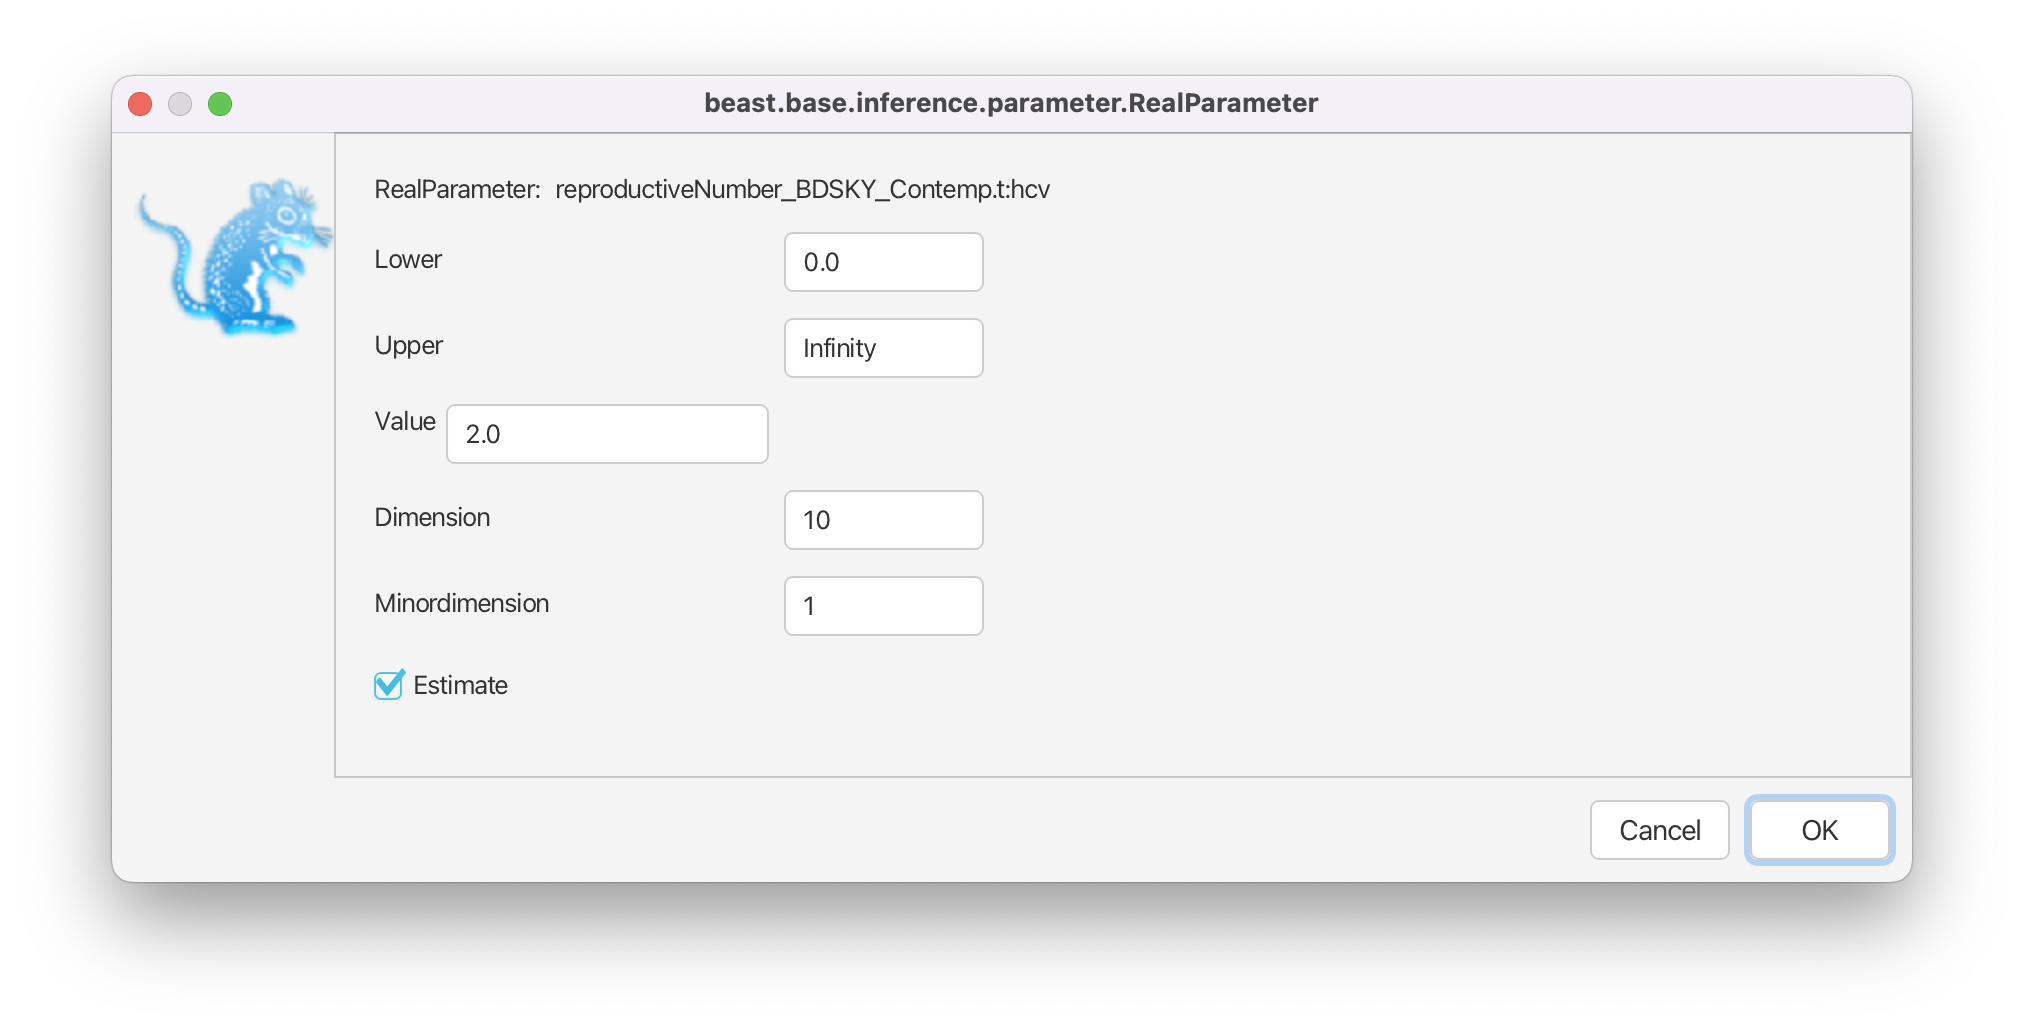
\includegraphics[width=0.750000\textwidth]{figures/choose_dimension_bdsky.png}
    \caption{Setting the dimension of the reproductiveNumber parameter.}
    \label{fig:dimensions_bdsky}
\end{figure}

This means that \passthrough{$ R_e $} will be allowed to
change at 9 equally spaced times between the origin of the epidemic and
the present time. Choosing this dimension can again be arbitrary and may
require the testing of a few different values. Too few intervals and not
all rate shifts are captured. Too many intervals and the intervals may
not contain enough information to infer parameters. (As with setting the
dimension of the Coalescent Bayesian Skyline the dimension of
\passthrough{$ R_e $} can also be set in the initialization
panel).

Besides \passthrough{$ R_e $}
(\textbf{reproductiveNumber}), the \textbf{Birth Death Skyline
Contemporary} model has 3 more parameters,
\textbf{becomeUninfectiousRate} (the rate at which infected patients
become uninfectious, \passthrough{$ \delta $}, through
recovery, death or isolation), \textbf{rho} (the proportion of lineages
sampled in the present, \passthrough{$ \rho $}) and the
\textbf{origin} (the time at which the index case became infected, which
is always earlier than the tMRCA of the tree). We may know some of these
parameters from literature or be able to estimate them from external
sources. For example, the average time that patients are able to
transmit a disease is informative about the
\textbf{becomeUninfectiousRate}. This prior knowledge we can incorporate
in our analysis by setting appropriate priors for these parameters.

We will use a lognormal prior for \passthrough{$ R_e $}.
This is a good prior distribution to use for rates since it is always
positive (a rate cannot be negative) and has a long tail defined over
all positive numbers. The long tail allows arbitrarily high estimates of
\passthrough{$ R_e $}, but does not place much weight on
very high rates. This agrees with our prior knowledge about
\passthrough{$ R_e $} (most diseases have an
\passthrough{$ R_e $} between 1.2 and 5. Measles is one of
the most infectious diseases we know about and has
\passthrough{$ R_e \approx 18 $}). If an epidemic is
neither growing or declining, it has an
\passthrough{$ R_e $} of 1, which we will use as a null
hypothesis, by setting a prior on \passthrough{$ R_e $}
centered around 1 (we assume that if there isn't a strong signal in an
interval for an epidemic to grow or decline that
\passthrough{$ R_e = 1 $}, i.e.~the epidemic size stays
constant). Note that this prior is used for each of the
\passthrough{$ R_e $} intervals (the Birth-Death Skyline
assumes that \passthrough{$ R_e $} is independent in each
of the intervals).

\begin{framed}
Select a \textbf{Log Normal} distribution for the
\textbf{reproductiveNumber} prior.

Click on the arrow to the left of \textbf{reproductiveNumber} to open
all the options for \passthrough{$ R_e $} settings

Set \textbf{M} to 0, which results in a median of 1. We set \textbf{S}
to 1.25, which places most weight below 7.82 (95\% quantile). (Figure
\ref{fig:r0prior}).
\end{framed}

\begin{figure}
    \centering
    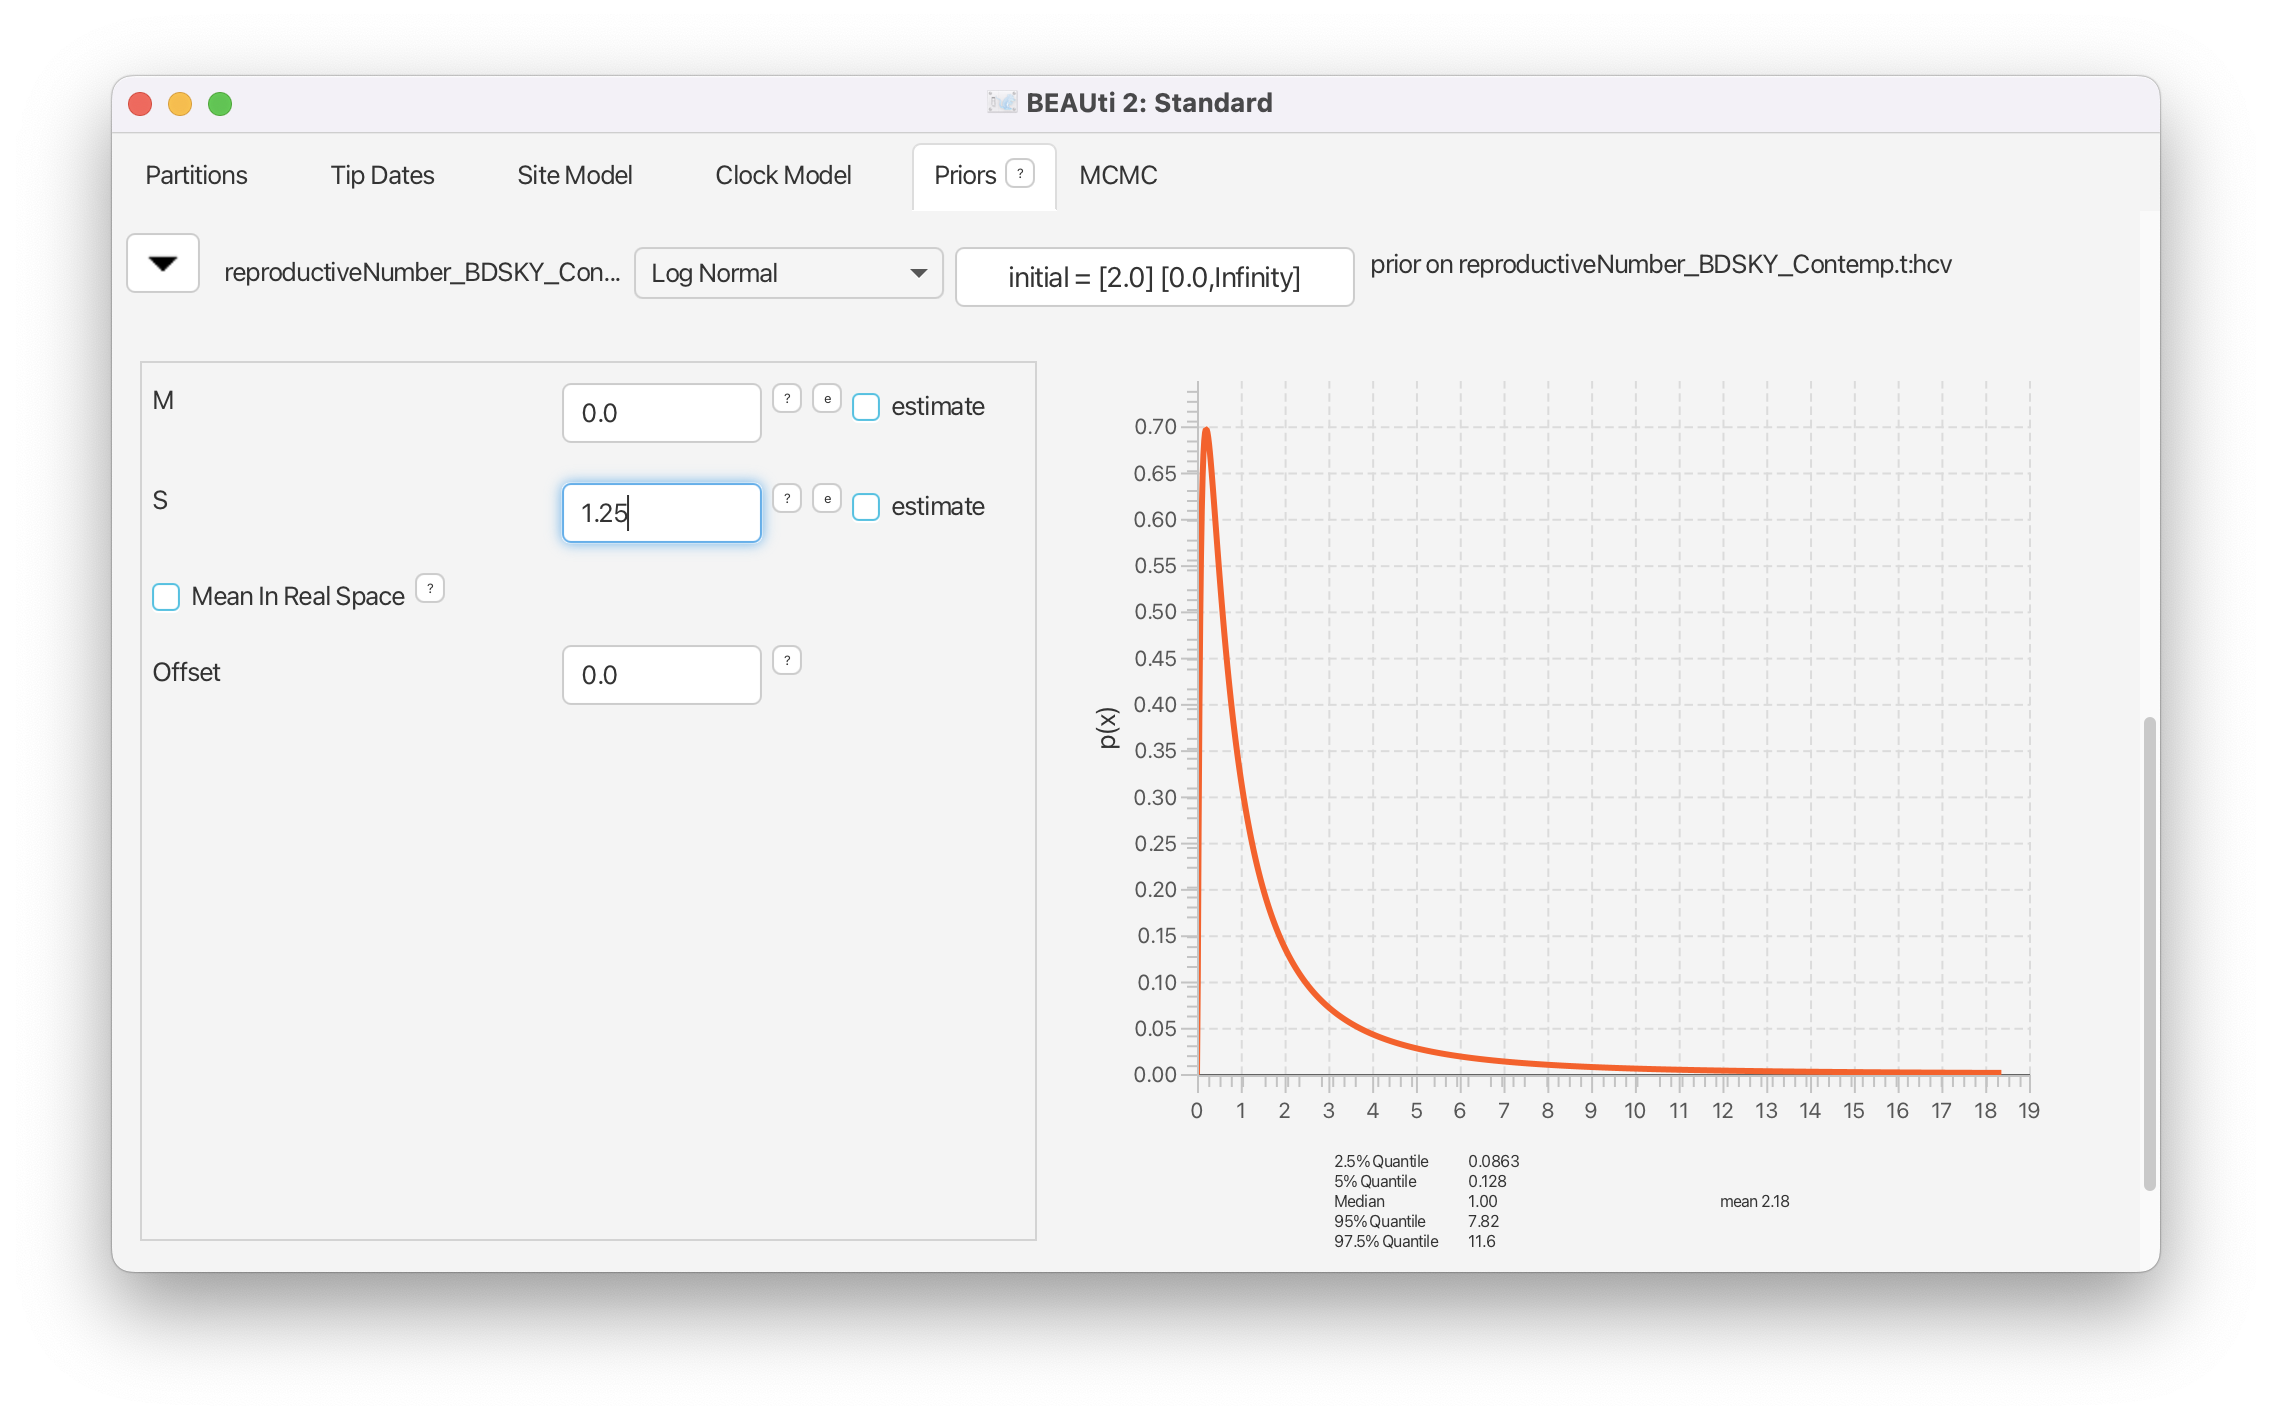
\includegraphics[max width=\textwidth, max height=0.9\textheight]{figures/bdsky_prior_r0.png}
    \caption{Setting the `$ R_e $` prior.}
    \label{fig:r0prior}
\end{figure}

For the becoming uninfectious rate we will again use a log normal prior.
The inverse of the becoming uninfectious rate is the average infectious
period. In some patients an HCV infection only lasts a few weeks, while
in others it is a chronic infection lasting for many years. Setting
\passthrough{$ M=0 $} and
\passthrough{$ S=1.25 $} results in the same prior we used
for the \passthrough{$ R_e $}. In terms of the becoming
uninfectious rate, this translates to the 95\% quantiles for the
infectious period falling between 0.0862 years (31.5 days) and 11.59
years, with a median of 1 year. We will see later that there is a strong
signal in the data for a longer becoming uninfectious period.

\begin{framed}
Set the same prior for \textbf{becomeUninfectiousRate} as for
\textbf{reproductiveNumber} (Log Normal, with M=0.0, S=1.25) (Figure
\ref{fig:bURprior})
\end{framed}

\begin{figure}
    \centering
    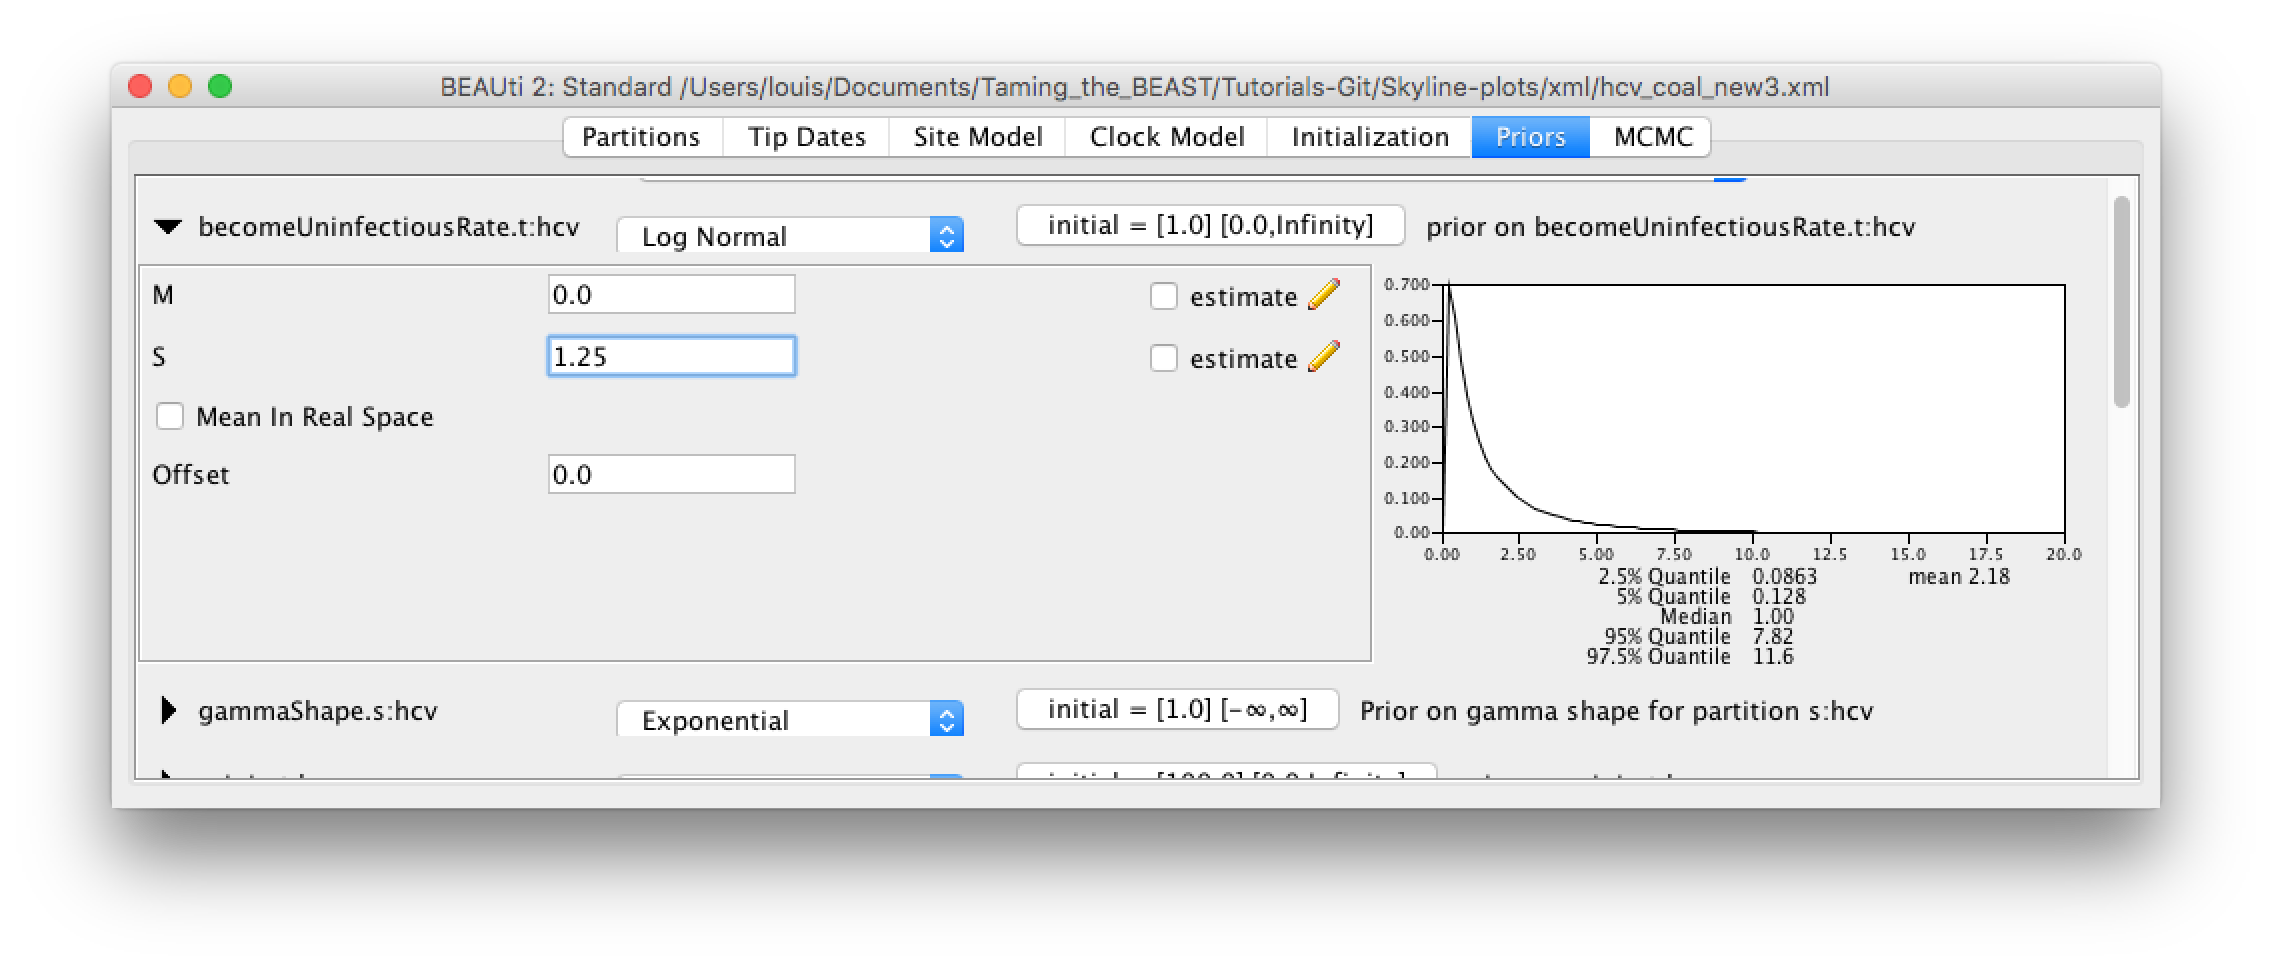
\includegraphics[max width=\textwidth, max height=0.9\textheight]{figures/bdsky_prior_uninf.png}
    \caption{Setting the becoming uninfectious rate prior.}
    \label{fig:bURprior}
\end{figure}

The sampling proportion, \passthrough{$ \rho $}, represents
the proportion of HCV cases in Egypt in 1993 that are included in the
analysis. In 1993 Egypt had a population of roughly 60 million people,
and with a prevalence of at least 15\% this translates into millions of
cases, while we only have 63 sequences.

We will use a beta distribution for the prior on
\passthrough{$ \rho $}. Beta distributions are a very
flexible class of distributions that are only defined between 0 and 1,
making them ideal to use for proportions.

\begin{framed}
Select a \textbf{Beta} distribution for the \textbf{rho} prior.

Click on the arrow to the left of \textbf{rho} to open all the options
for the prior settings.

Alpha to 1 and Beta to 9999, reflecting our prior knowledge that our
dataset represents only a miniscule fraction of cases (Figure
\ref{fig:rhoprior}).
\end{framed}

\begin{figure}
    \centering
    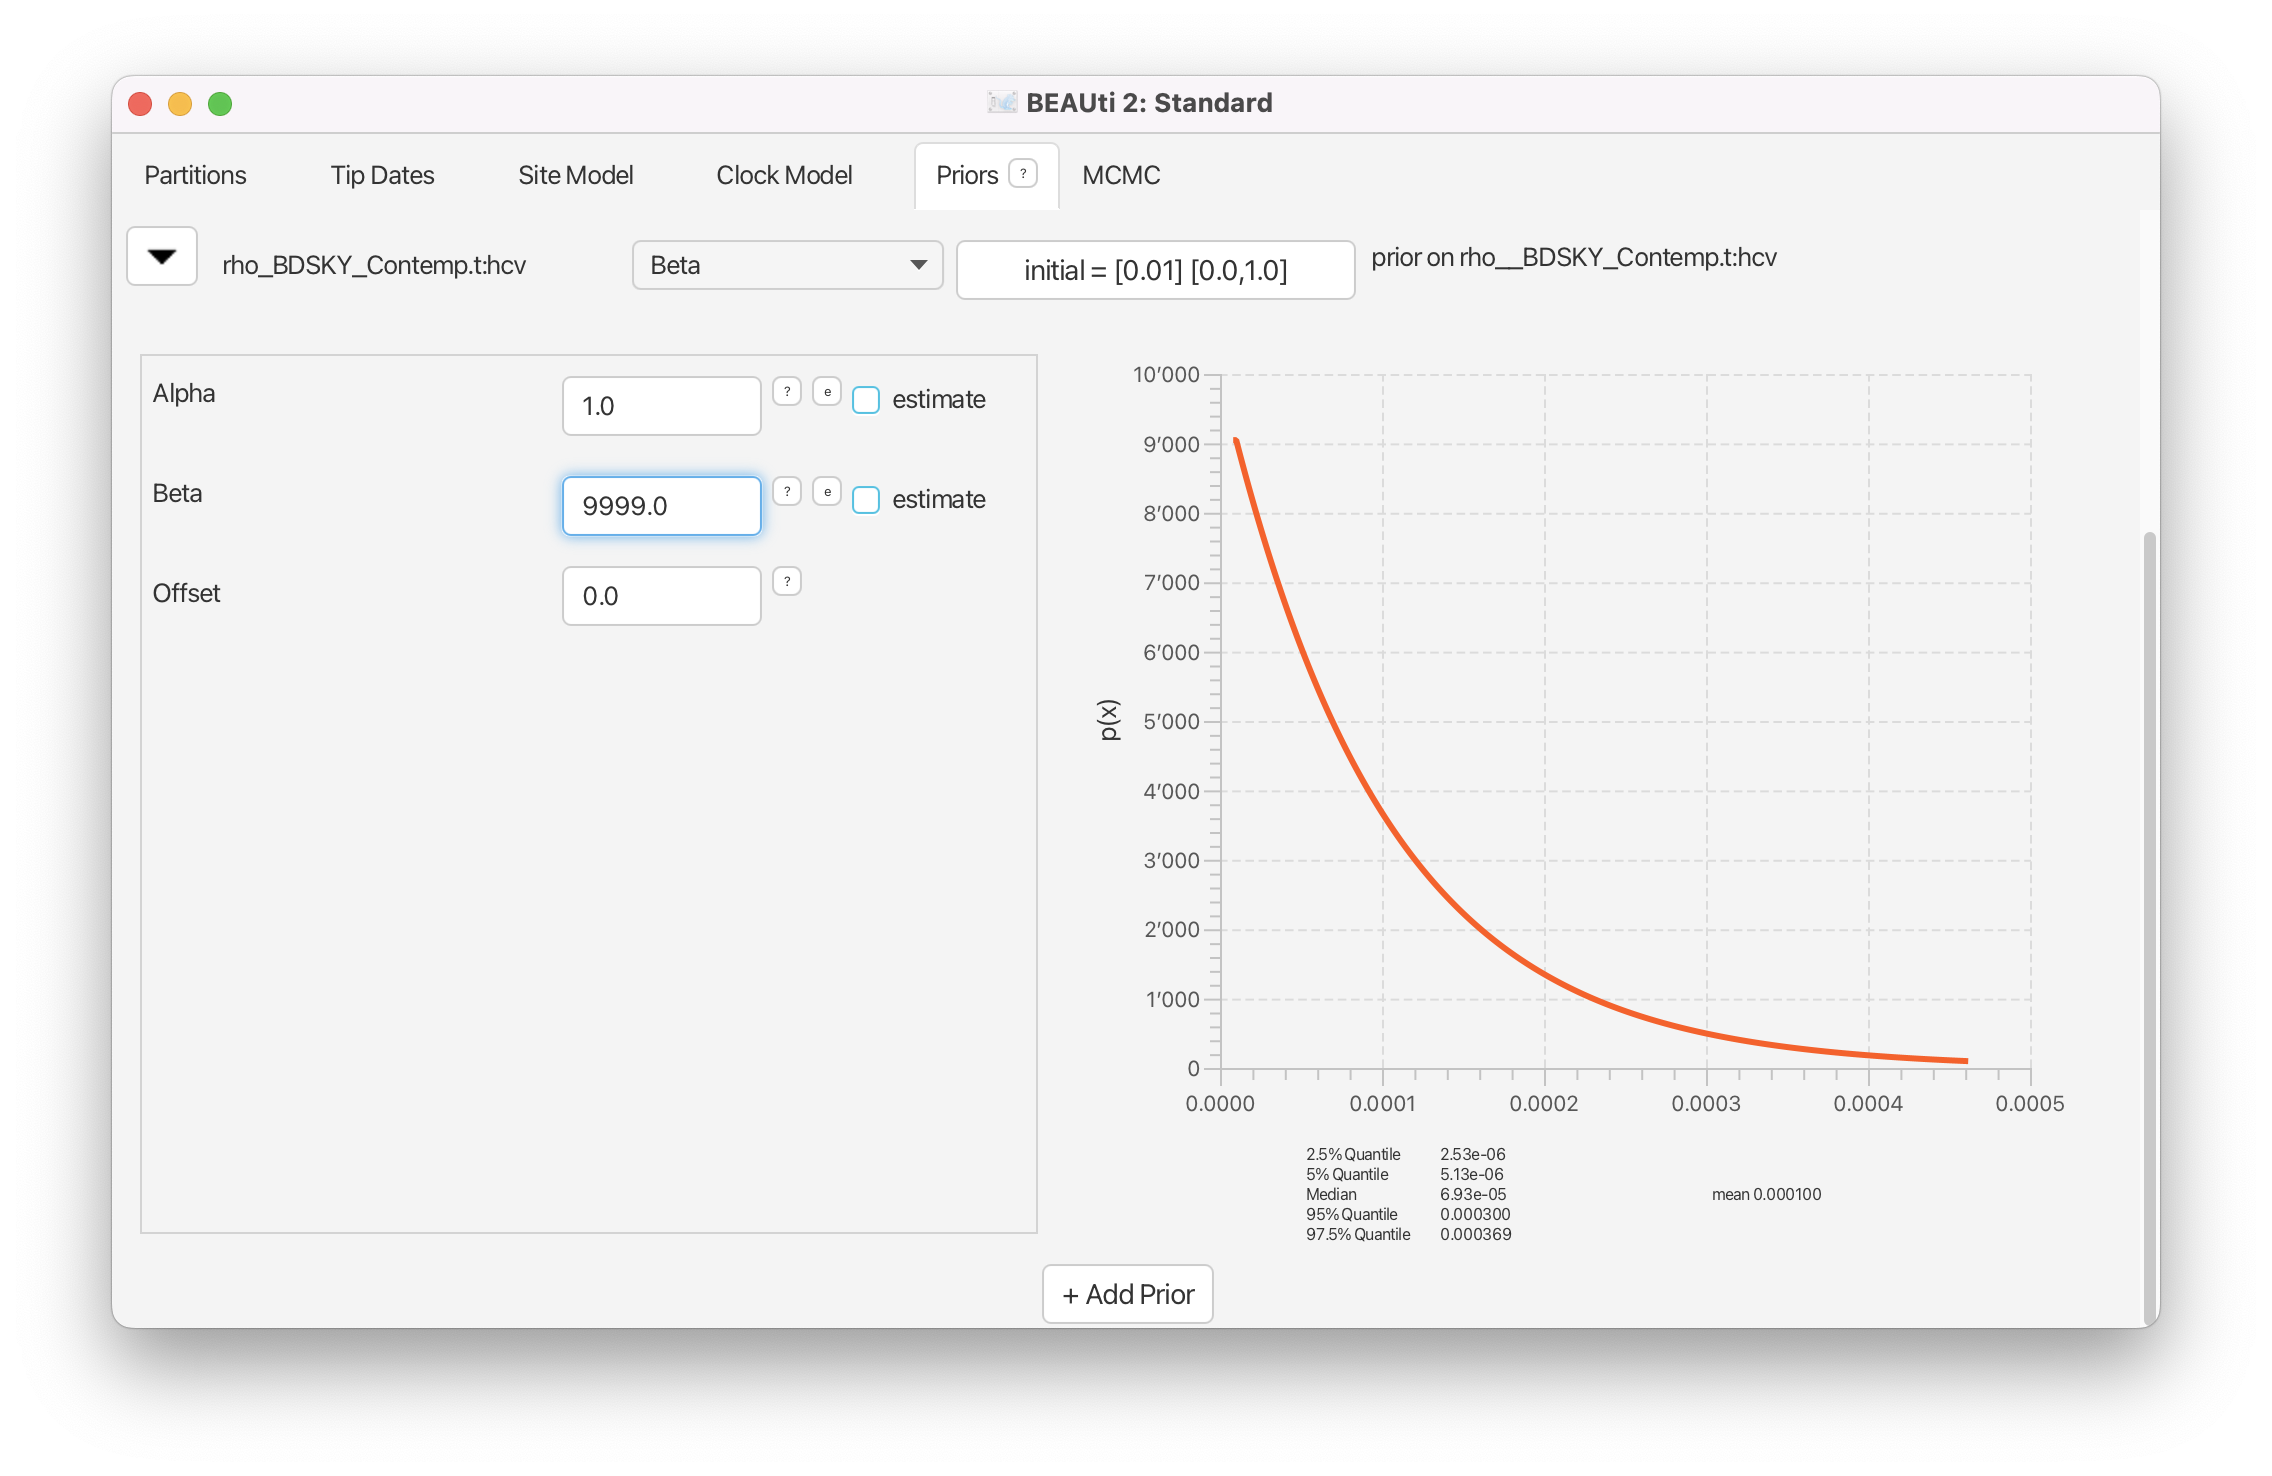
\includegraphics[max width=\textwidth, max height=0.9\textheight]{figures/bdsky_prior_rho.png}
    \caption{Setting the prior on `$ \rho $`.}
    \label{fig:rhoprior}
\end{figure}

Finally, we need to set a prior for the origin of the epidemic. We will
once again use a log normal distribution for this parameter. Note that
the origin also has to be positive and needs to be bigger than the MRCA
of the tree. We know that HCV has been circulating in Egypt for at least
a hundred years, so we set a prior with a median value greater than 100.

\begin{framed}
Set a \textbf{Log Normal} prior for \textbf{origin} with \textbf{M = 5}
and \textbf{S = 0.5} (Figure \ref{fig:oriprior}), resulting in a median
prior estimate for the origin of 148 years.
\end{framed}

\begin{figure}
    \centering
    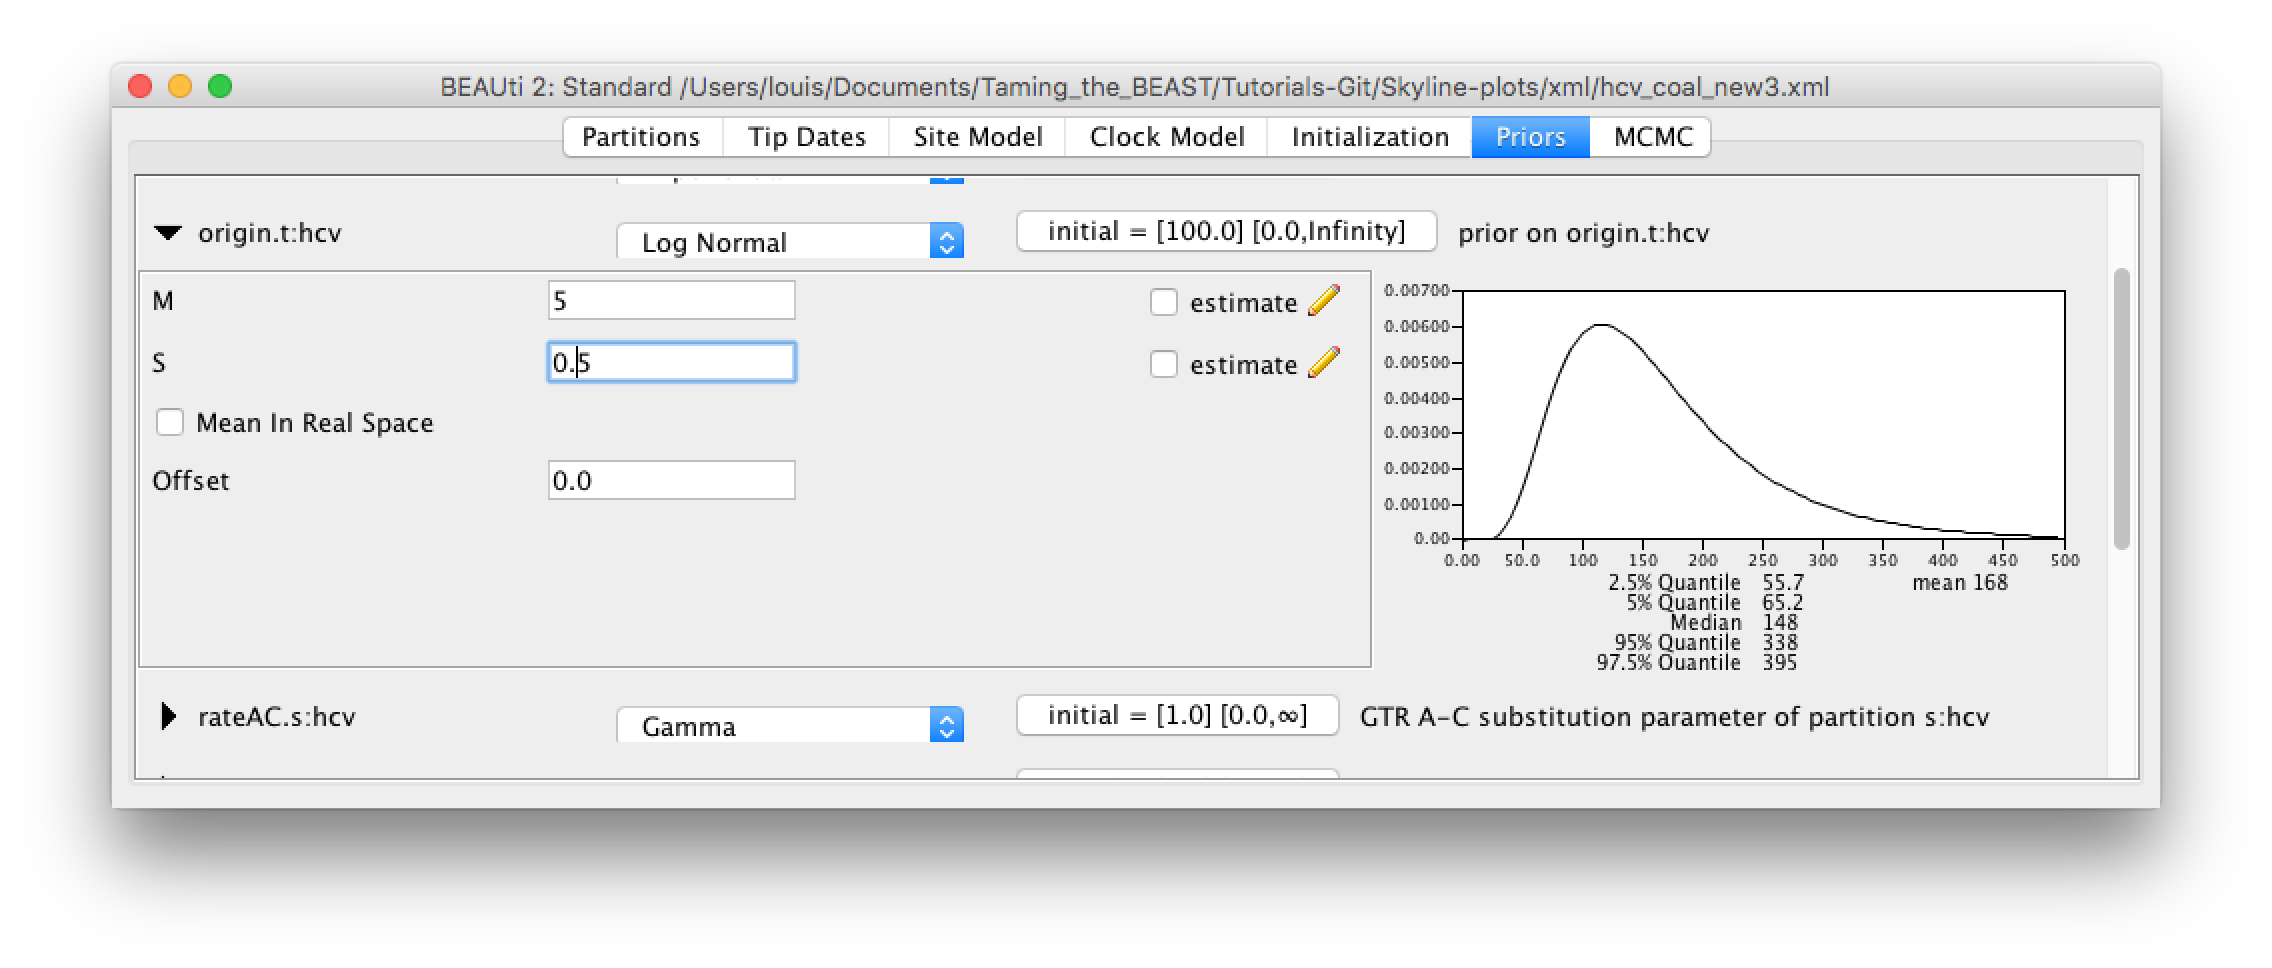
\includegraphics[max width=\textwidth, max height=0.9\textheight]{figures/bdsky_prior_ori.png}
    \caption{Setting the prior on the origin of the epidemic.}
    \label{fig:oriprior}
\end{figure}

The rest of the priors pertain to the site model parameters and we can
leave them as they are.

\begin{framed}
Navigate to the \textbf{MCMC} panel.

Change the \textbf{Chain Length} from 10'000'000 to 3'000'000.

Click on the arrow next to the \textbf{tracelog} and change the
\textbf{File Name} to \passthrough{lstinline!\$(filebase).log!} and set
the \textbf{Log Every} to 3'000.

Click on the arrow next to the \textbf{treelog} and change the
\textbf{File Name} to \passthrough{lstinline!\$(filebase)-\$(tree).log!}
and set the \textbf{Log Every} to 3'000.

Leave all other settings at their default values and save the file as
\passthrough{\lstinline!hcv_bdsky.xml!}.

(Note that since BEAST 2.7 the filenames used here are the default
filenames and should not need to be changed!)
\end{framed}

Now we are ready to run the analysis.

\begin{framed}
Start \textbf{BEAST2} and choose the file
\passthrough{\lstinline!hcv_bdsky.xml!}.

If you have \textbf{BEAGLE} installed tick the box to \textbf{Use BEAGLE
library if available}, which will make the analysis run faster.

Hit \textbf{Run} to start the analysis.
\end{framed}

Look at the topics for discussion below and read through the next
section while waiting for the analysis to finish.

\begin{framed}
\textbf{Topics for discussion:}

\begin{itemize}

\item
  We set a prior on \passthrough{$ R_e $} in the
  Birth-Death Skyline analysis, but did not set any prior for
  \passthrough{$ N_e $} in the Coalescent Bayesian Skyline
  analysis. Is there a prior on \passthrough{$ N_e $}? If
  so, what is it?
\item
  We fixed the clock rate to an independent estimate and set a strict
  clock. If we had strong prior knowledge that there is substitution
  rate variation over time in the Egyptian HCV epidemic, could we use a
  relaxed clock here?
\end{itemize}
\end{framed}

\hypertarget{the-birth-death-skyline-parameterization}{%
\subsubsection{The Birth-Death Skyline
parameterization}\label{the-birth-death-skyline-parameterization}}

The birth-death model is parameterized very differently from the
coalescent model, using per lineage rates and an explicit sampling model
(whereas the coalescent model conditions on the samples). This makes the
birth-death model more powerful, but also much more complex. A basic
birth-death model has a birth rate
(\passthrough{$ \lambda $}), the rate at which lineages are
added to the tree, and a death rate
(\passthrough{$ \delta $}), the rate at which lineages are
removed from the tree (Figure \ref{fig:bd_model}). In an infectious
disease epidemic \passthrough{$ \lambda $} can be thought
of as the transmission rate, the rate at which infected individuals
infect susceptibles, while \passthrough{$ \delta $} can be
thought of as the becoming uninfectious rate, the rate at which infected
individuals recover, die or are isolated. In species tree inferences
these rates can be thought of in terms of speciation and extinction.

\begin{figure}
    \centering
    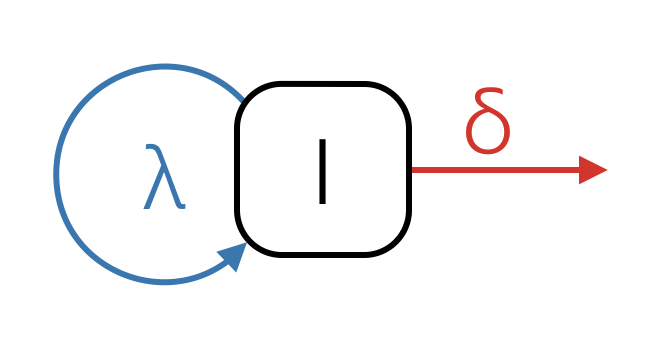
\includegraphics[width=0.250000\textwidth]{figures/bd_model.png}
    \caption{A schematic of the birth-death model.}
    \label{fig:bd_model}
\end{figure}

The \textbf{Birth Death Skyline Contemporary} model we used was
parameterized in terms of \passthrough{$ R_e $} and
\passthrough{$ \delta $}. Recall that
\passthrough{$ R_e > 1 $} means that an epidemic will keep
growing. We can see this from the definition of
\passthrough{$ R_e $} as the ratio of the birth and death
rates.

\begin{equation}
    R_{e} = \frac{\lambda}{\delta}
\end{equation}

if \passthrough{$ \lambda > \delta $} then
\passthrough{$ R_e > 1 $}

epidemic grows

if \passthrough{$ \lambda = \delta $} then
\passthrough{$ R_e = 1 $}

epidemic stays constant

if \passthrough{$ \lambda < \delta $} then
\passthrough{$ R_e < 1 $}

epidemic declines

We used this paramerization simply because it is often easier to specify
priors for \passthrough{$ R_e $} than the transmission
rate, and because \passthrough{$ R_e $} is often more
informative for prevention efforts. In addition, the model also has a
sampling probability (\passthrough{$ \rho $}) parameter,
which in our analysis describes how likely it is that a person infected
with HCV in Egypt in 1993 was sampled in our dataset. The final
parameter is the origin. Whereas coalescent models work backward-in-time
from the sampled sequences, birth-death models work forward-in-time from
the origin. Hence, the model needs an origin time, which can also be
jointly estimated along with the other parameters. The origin will
always be at least as big, and usually bigger, than the tMRCA of the
sampled tree, since the sampled tree is by definition smaller than the
complete tree.

You may have noticed that there are many Birth-Death Skyline models
available in BEAUti. For example, the \textbf{Birth Death Skyline
Contemporary BDSParam} model is parameterized in terms of
\passthrough{$ \lambda, \delta $} and
\passthrough{$ \rho $} and is usually more appropriate for
macroevolutionary studies. The \textbf{Birth Death Skyline Serial} model
assumes that the data are heterochronous (sampled at different times).
It assumes that:

\begin{equation}
    \delta = \psi + \mu
\end{equation}

where \passthrough{$ \psi $} is the rate at which lineages
are sampled through time and \passthrough{$ \mu $} is the
rate at which lineages are removed from the tree for any other reason
(death, recovery, extinction etc.). (In this case the
\passthrough{$ \rho $} parameter is no-longer available by
default, because samples are collected through time, and not just at one
timepoint). By default, the model is parameterized in terms of
\passthrough{$ R_e , \delta $} and
\passthrough{$ p $}, the sampling proportion:

\begin{equation}
    p = \frac{\psi}{\psi + \mu}
\end{equation}

The sampling proportion is the proportion of all removed lineages that
were sampled, and can be used to obtain a rough estimate of the total
population size. This model is useful for studying infectious disease
dynamics, because samples are often collected over the course of an
epidemic. It can also be used for macro-evolutionary studies, when
fossil data (morphological traits or ancient DNA) are incorporated. In
that case a parameterization in terms of
\passthrough{$ \lambda, \mu $} and
\passthrough{$ \psi $} is preferable.

You can also see that the model \textbf{Birth Death Skyline Serial}
assumes that upon sampling a lineage is removed from the tree (e.g.~in a
disease model the sampled individual cannot transmit the disease after
sampling). The consequence for the phylogeny is that a sampled lineage
cannot be a direct ancestor of any other lineage in the tree. This
assumption can be relaxed, but we will not do so during this tutorial.

The Birth-Death Skyline model is very flexible and allows any or all of
these rates to change independently over time. This is done by dividing
the time from the origin to the most recent sample into dimension
\passthrough{$ d $} equally spaced intervals (see Figure
\ref{fig:bdsky_principle}). The rates are then allowed to change between
intervals. Since some rates (e.g.~\passthrough{$ \lambda $}
and \passthrough{$ \delta $}) are highly correlated, it is
not always a good idea to let all rates change over time because it can
lead to poor mixing or biased estimates (often we assume that the
becoming uninfectious rate is constant while allowing
\passthrough{$ R_e $} to change over time, as we did here).
It is also possible to specify the change-point times more flexibly, or
even estimate them, however for now this requires editing the XML file.
Some examples are available
\href{https://github.com/laduplessis/skylinetools/wiki/TreeSlicer}{here}.

\begin{figure}
    \centering
    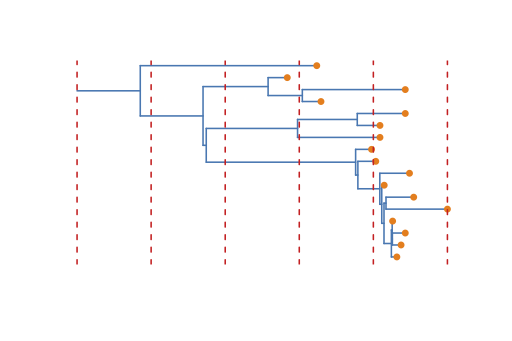
\includegraphics[width=0.750000\textwidth]{figures/bdsky_intervals5.png}
    \caption{Example tree where the red dotted lines are an example of where rates could be allowed to change on the tree. The branch at the root (compare Figure 6) is indicating the origin of the epidemic, which is also estimated in the BDSKY.}
    \label{fig:bdsky_principle}
\end{figure}

\hypertarget{visualizing-the-birth-death-skyline-output}{%
\subsubsection{Visualizing the Birth-Death Skyline
Output}\label{visualizing-the-birth-death-skyline-output}}

There is no equivalent built-in visualization of the skyline plot of a
Birth-Death Skyline (BDSKY) analysis in Tracer as there is for the
Coalescent Bayesian Skyline. But because BDSKY separates the full tree
into equally spaced intervals, we can already get an idea of the
inference just by looking at the inferred
\passthrough{$ R_e $} values (see Figure
\ref{fig:bdsky_dynamics}). This gives us a good idea of the trend, but
it is not completely accurate. Since we are also estimating the origin
parameter, the interval times are slightly different in each posterior
sample and overlap slightly. The advantage of this is that we get a
smooth estimate through time. The disadvantage is that we need to do
some extra post-processing to plot the smooth skyline.

As with the Coalescent Bayesian Skyline, because we shortened the chain,
most parameters have very low ESS values. If you like, you can compare
your results with the example results we obtained with identical
settings and a chain of 30,000,000
(\passthrough{\lstinline!hcv_bdsky_30M.log!}).

\begin{figure}
    \centering
    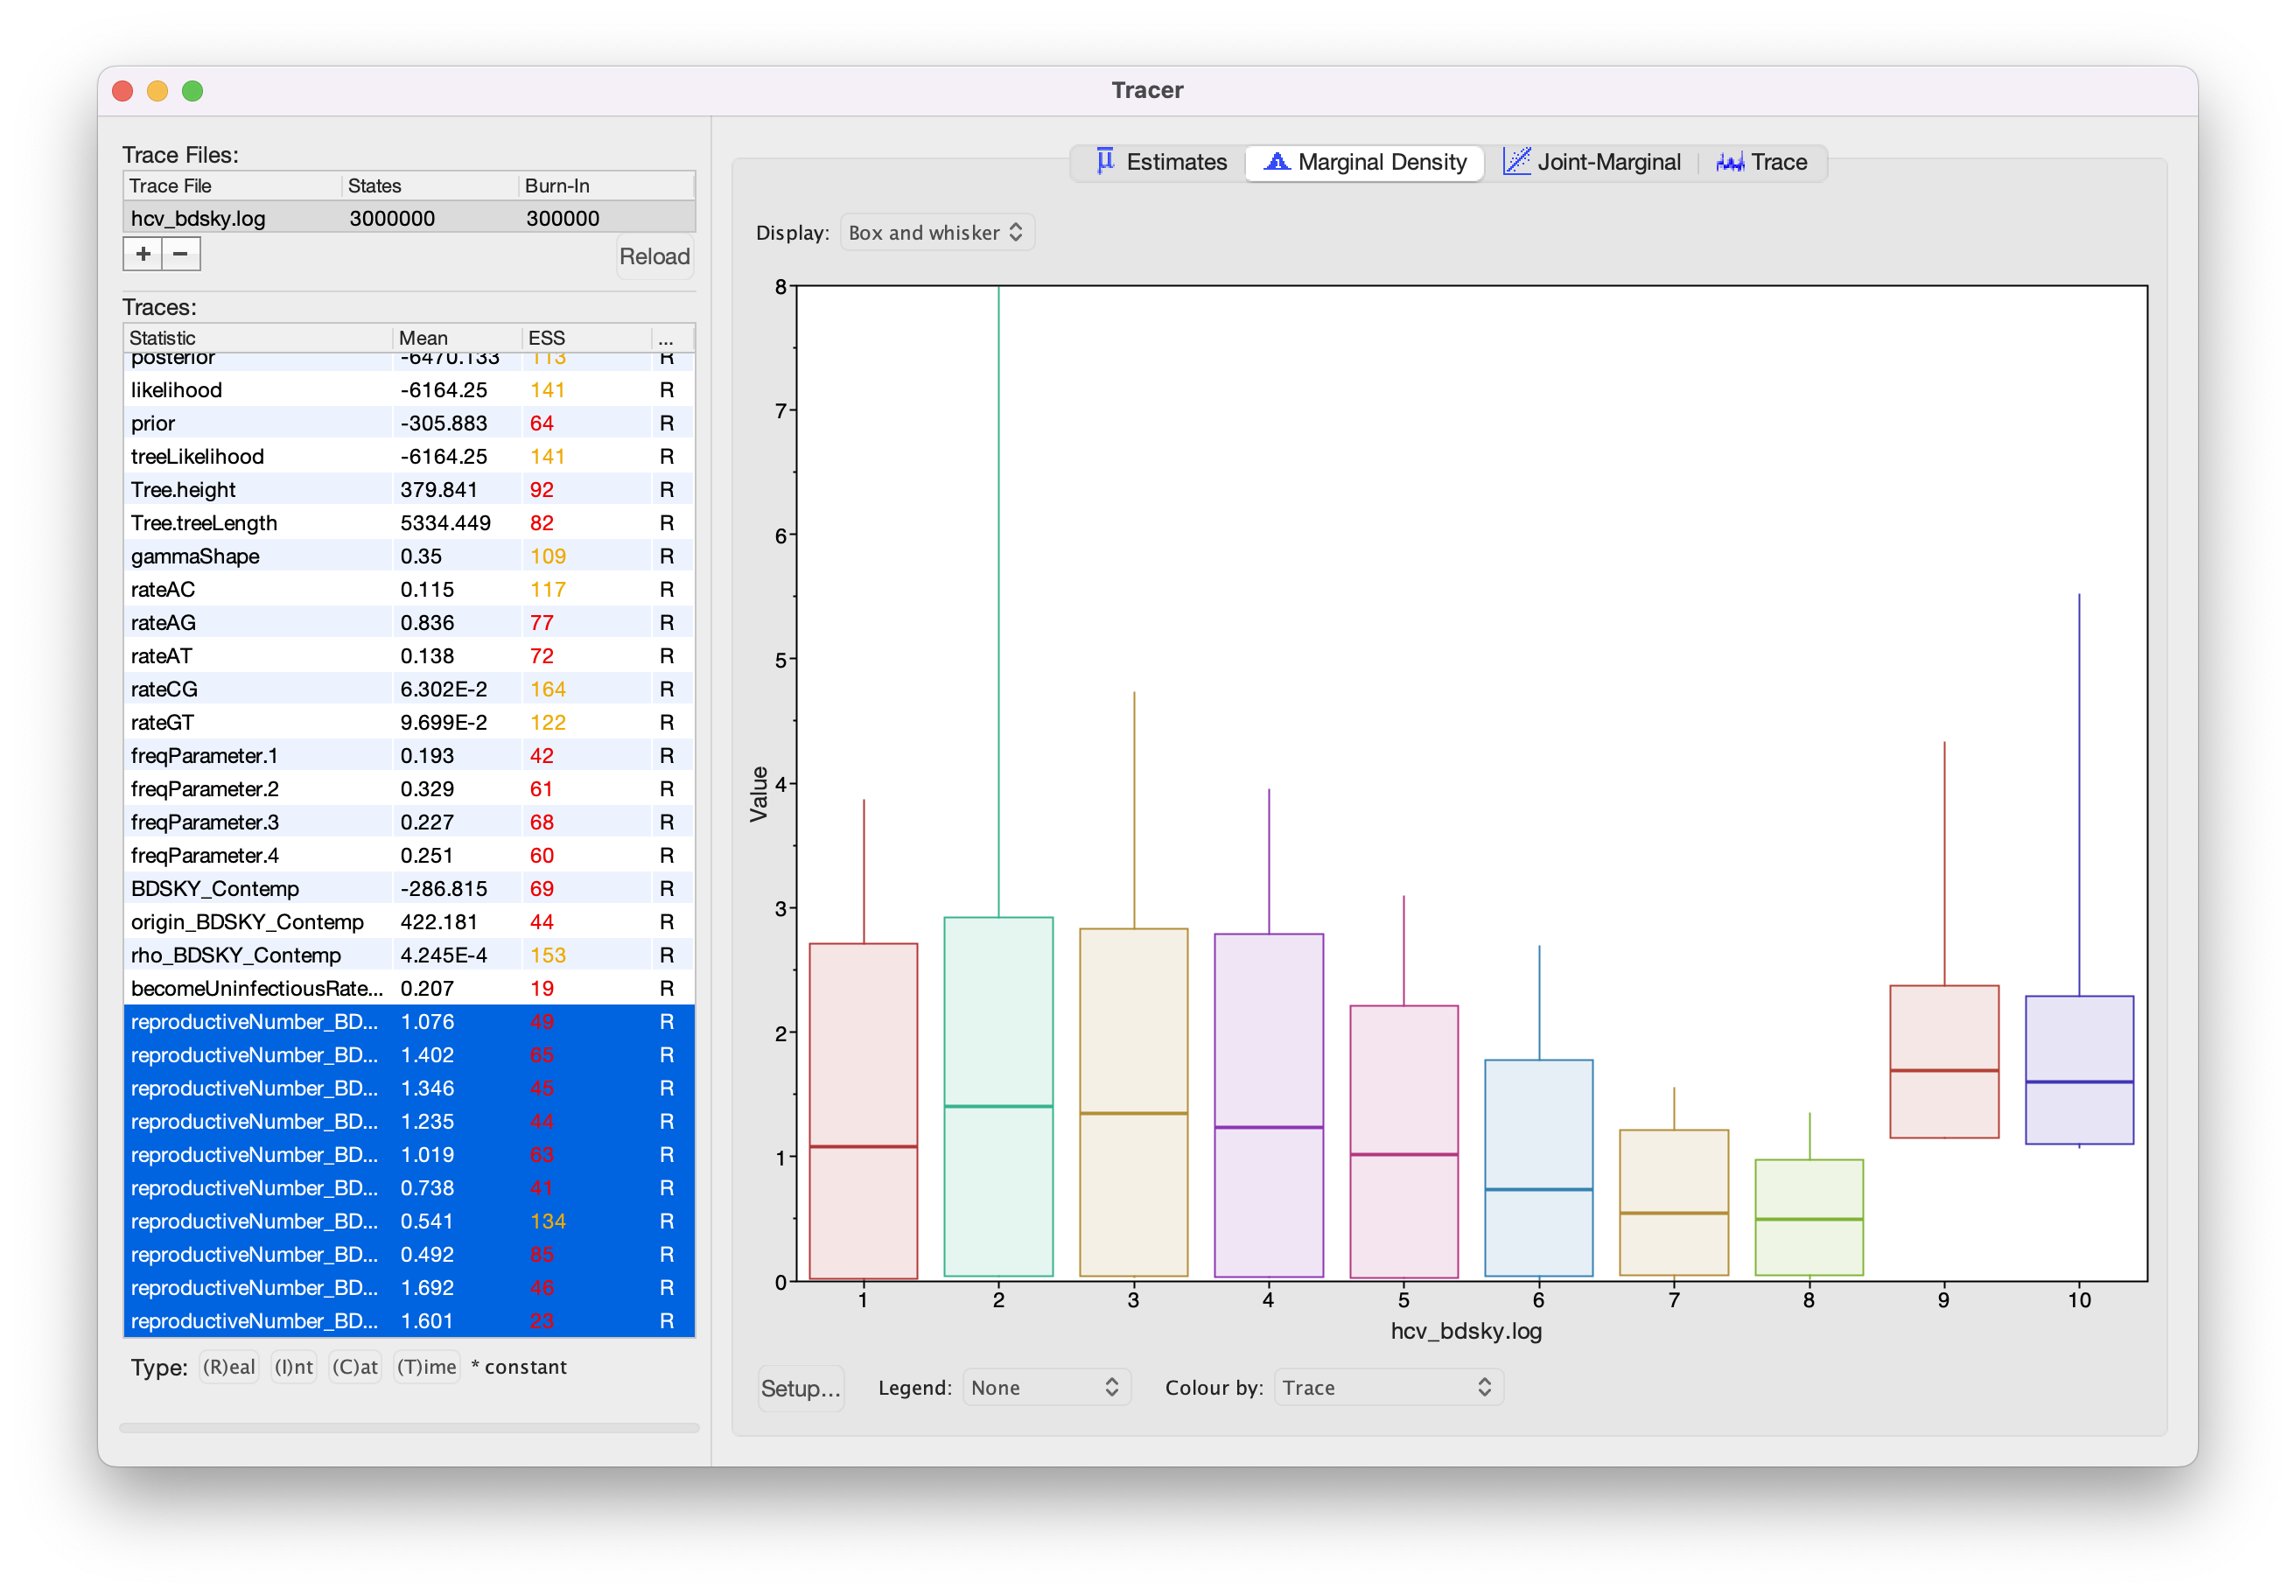
\includegraphics[max width=\textwidth, max height=0.9\textheight]{figures/bdsky_tracer.png}
    \caption{Estimated population dynamics by BDSKY in Tracer.}
    \label{fig:bdsky_dynamics}
\end{figure}

We will use R to post-process and plot the Birth-Death Skyline. The
below steps are also in an RMarkDown notebook on the left-hand panel,
under the heading \textbf{Scripts}.

First, install the necessary packages. Once installed, we don't need to
install the packages again. Because two of the packages we need are not
available on CRAN we install them from GitHub.

\begin{lstlisting}
install.packages("devtools")
install.packages("coda")
devtools::install_github("laduplessis/bdskytools")
devtools::install_github("laduplessis/beastio")
\end{lstlisting}

Once the packages are installed we have to load them into our R
workspace before we can use their functions.

To plot the results, we need to first tell R where to find the
\passthrough{\lstinline!*.log!} file of our run and then load it into R
(discarding 10\% of samples as burn-in). If you are using RStudio, you
can change the working directory to the directory where you stored your
log files, which makes it easier to load the files in R. In the
RMarkDown notebook the logfile location is stored in the
\passthrough{\lstinline!params$logfile!} parameter.

\begin{lstlisting}
library(coda)
library(bdskytools)
library(beastio)

bdsky_trace   <- beastio::readLog(params$logfile, burnin=0.1)
\end{lstlisting}

With the trace loaded as an \passthrough{\lstinline!mcmc!} object from
the coda package we can use coda functions to investigate the trace and
check convergence. For details on how to use coda see the package on
\href{https://cran.r-project.org/web/packages/coda/index.html}{CRAN}.

Next, we can extract the HPDs of \passthrough{$ R_e $} and
the becoming uninfectious rate:

\begin{lstlisting}
Re_sky    <- beastio::getLogFileSubset(bdsky_trace, "reproductiveNumber_BDSKY_Contemp")
Re_hpd    <- t(beastio::getHPDMedian(Re_sky))
delta_hpd <- beastio::getHPDMedian(bdsky_trace[, "becomeUninfectiousRate_BDSKY_Contemp"])
\end{lstlisting}

Next we plot the raw HPD intervals of
\passthrough{$ R_e $}. This is equivalent to the output in
Tracer.

\begin{lstlisting}
bdskytools::plotSkyline(1:10, Re_hpd, type='step', ylab="R")
\end{lstlisting}

\begin{figure}
    \centering
    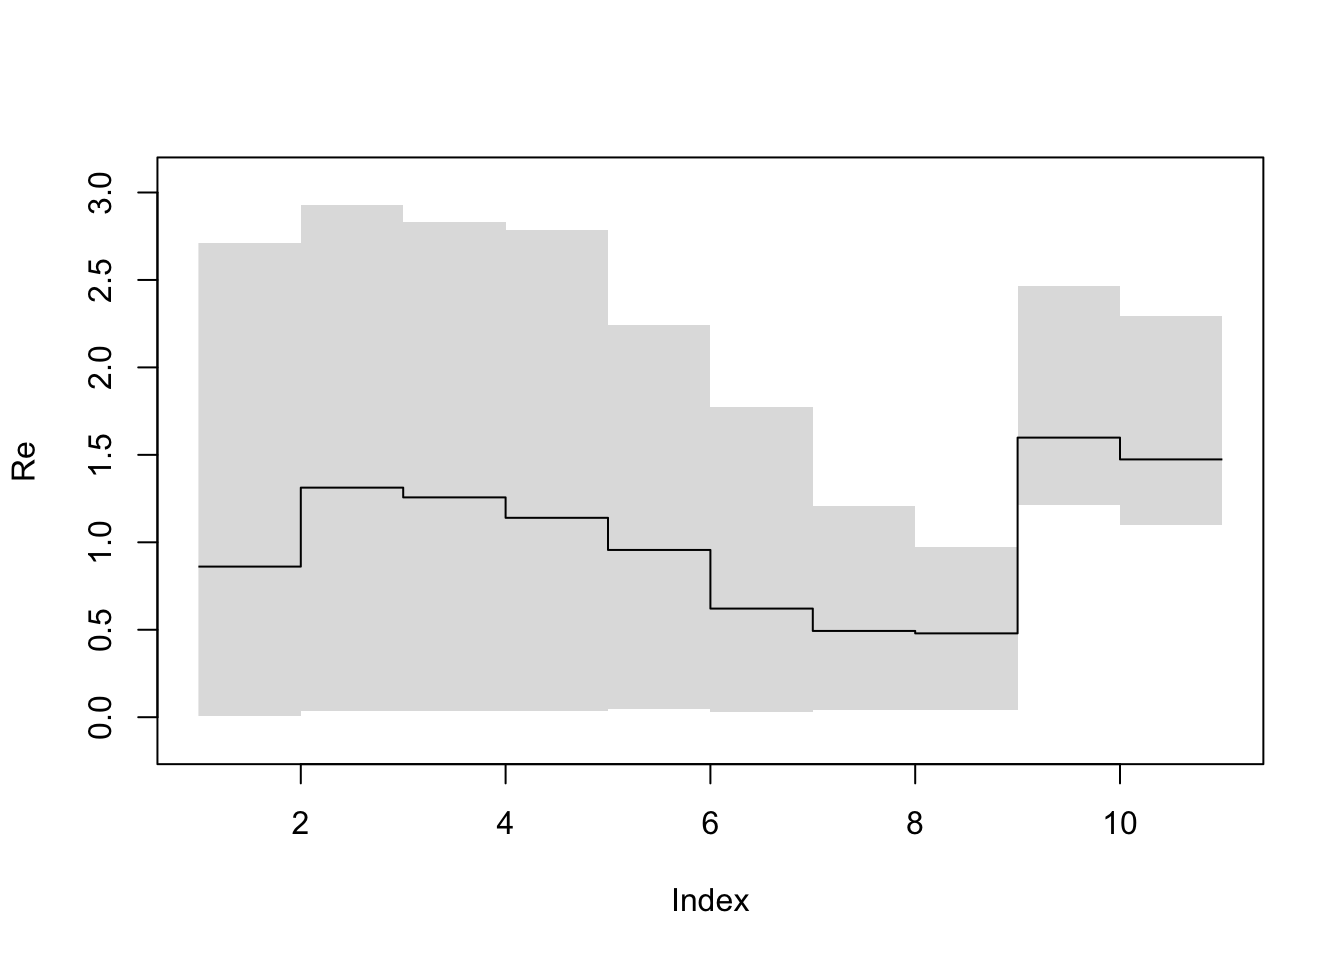
\includegraphics[width=0.800000\textwidth]{scripts/figs/plot-Re-ungridded-1.png}
    \caption{The HPDs of `$ R_e $` (equivalent to the previous figure from Tracer).}
    \label{fig:bdsky_hpds}
\end{figure}

In order to plot the smooth skyline we have to marginalise our
$R_e $ estimates on a regular timegrid and
calculate the HPD at each gridpoint. It is usually a good idea to use a
grid with more cells than the dimension of
$R_e$ (but using too many can result in
noisy estimates). To do this we first calculate the marginal posterior
at every time of interest using the function
\passthrough{\lstinline!bdskytools::gridSkyline!} and then calculate the
HPD for each of the finer time intervals. Here we choose to look at
\passthrough{\lstinline!params$gridsize!} equidistantly spaced points
between the median tMRCA and the most recent sequence. The times to grid
the skyline on (\passthrough{\lstinline!timegrid!}), refers to years in
the past.

\begin{lstlisting}[language=R]
tmrca_med  <- median(bdsky_trace[, "Tree.height"])
gridTimes  <- seq(0, median(tmrca_med), length.out=params$gridsize)  
    
Re_gridded <- mcmc(bdskytools::gridSkyline(Re_sky, bdsky_trace[, "origin_BDSKY_Contemp"], gridTimes))
Re_gridded_hpd <- t(getHPDMedian(Re_gridded))
\end{lstlisting}

Now we are ready to plot the smooth skyline (remember that the sequences
were sampled in 1993):

\begin{lstlisting}[language=R]
times <- 1993 - gridTimes
plotSkyline(times, Re_gridded_hpd, xlab="Date", ylab="Re", type="smooth") 
\end{lstlisting}

\begin{figure}
    \centering
    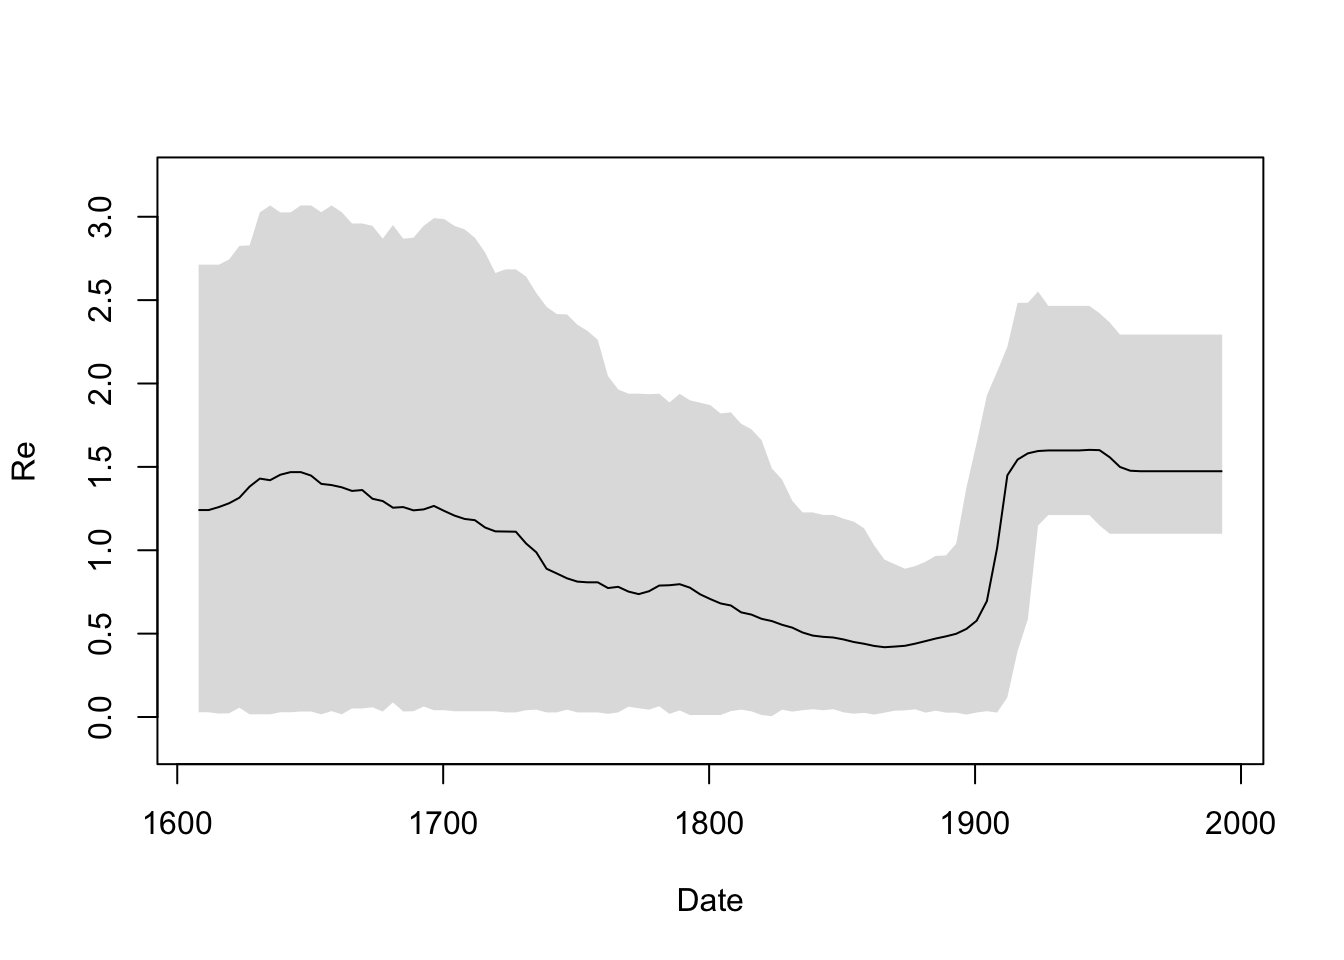
\includegraphics[width=0.800000\textwidth]{scripts/figs/plot-Re-1.png}
    \caption{The smooth `$ R_e $` skyline.}
    \label{fig:bdsky_smooth}
\end{figure}

We can plot the gridded $R_e$ skyline (not
its HPDs) for a few of the states in our MCMC chain to see what it
really looks like as the Markov chain samples parameters. Note that the
intervals overlap between different posterior samples. This is because
the origin estimate is a different sample from the origin's posterior
density in each of the plotted samples. As we add more samples to the
plot we start to see the smooth skyline appear.

\begin{lstlisting}[language=R]
plotSkyline(times, Re_gridded, type='steplines', traces=1, col=pal.dark(cblue,1),ylims=c(0,5), 
            xlab="Time", ylab="R", main="1 random sample")
plotSkyline(times, Re_gridded, type='steplines', traces=10, col=pal.dark(cblue,0.5),ylims=c(0,5), 
            xlab="Time", ylab="R", main="10 random samples")
plotSkyline(times, Re_gridded, type='steplines', traces=100, col=pal.dark(cblue,0.5),ylims=c(0,5), 
            xlab="Time", ylab="R", main="100 random samples")
plotSkyline(times, Re_gridded, type='steplines', traces=1000, col=pal.dark(cblue,0.1),ylims=c(0,5), 
            xlab="Time", ylab="R", main="1000 random samples")
\end{lstlisting}

\begin{figure}
    \centering
    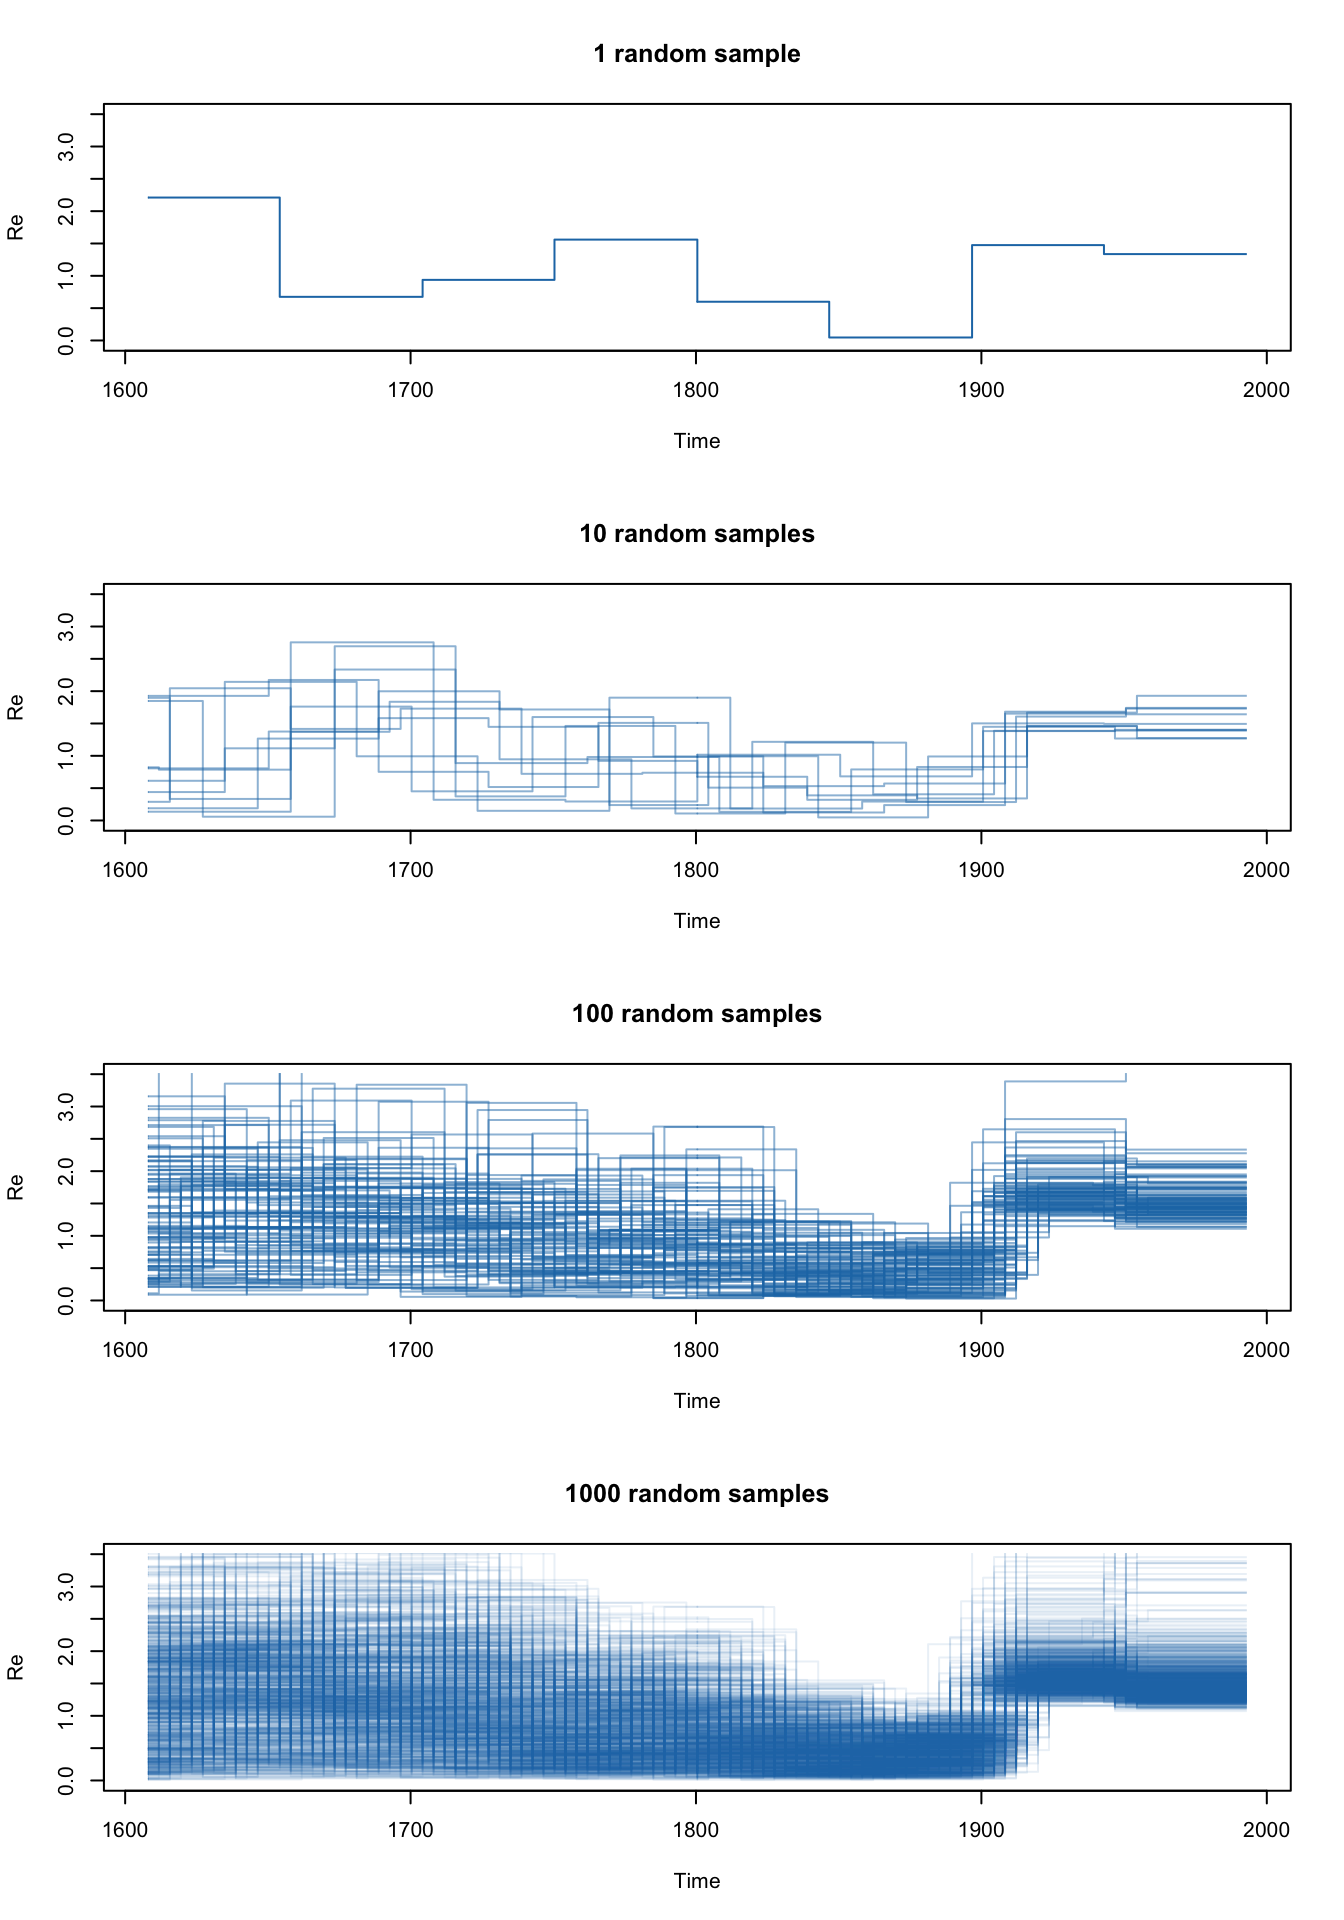
\includegraphics[width=0.800000\textwidth]{scripts/figs/plot-Re-traces-1.png}
    \caption{Increasing the number of traces plotted from 1 to 10, to 100, to 1000.}
    \label{fig:bdsky_traces}
\end{figure}

Finally, we can plot both the \passthrough{$ R_e $} and
\passthrough{$ \delta $} (the becoming uninfectious rate)
on a single set of axes. Since we left the dimension of the becoming
uninfectious rate at 1, it is constant through time. (Normally we would
not plot constant parameters over a time period)! The output should be
similar to Figure \ref{fig:bdsky_out}.

\begin{lstlisting}[language=R]
par(mar=c(5,4,4,4)+0.1)

plotSkylinePretty(range(times), as.matrix(delta_hpd), type='step', axispadding=0.0, 
                  col=pal.dark(cblue), fill=pal.dark(cblue, 0.5), col.axis=pal.dark(cblue), 
                  ylab=expression(delta), side=4, yline=2, ylims=c(0,1), xaxis=FALSE)

plotSkylinePretty(times, Re_gridded_hpd, type='smooth', axispadding=0.0, 
                  col=pal.dark(corange), fill=pal.dark(corange, 0.5), col.axis=pal.dark(corange), 
                  xlab="Time", ylab=expression("R"[e]), side=2, yline=2.5, xline=2, xgrid=TRUE, 
                  ygrid=TRUE, gridcol=pal.dark(cgray), ylims=c(0,3), new=TRUE, add=TRUE)
\end{lstlisting}

\begin{figure}
    \centering
    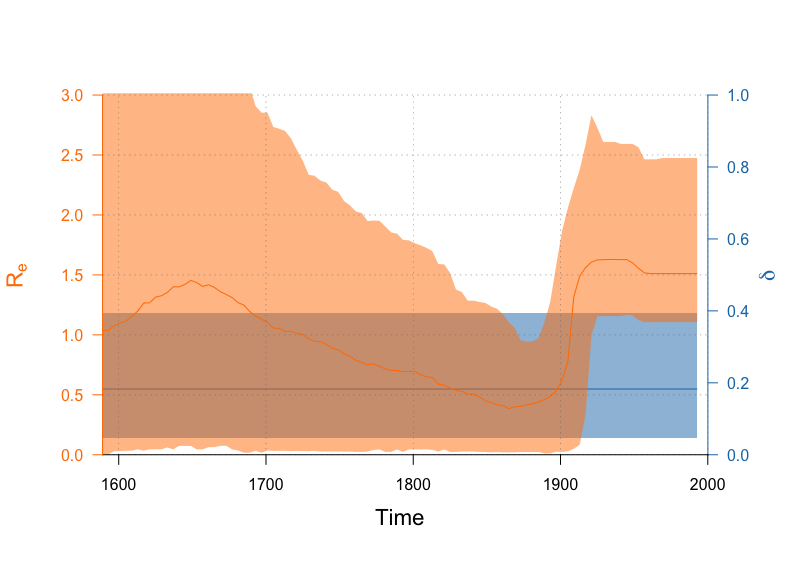
\includegraphics[width=0.800000\textwidth]{figures/bdsky_output_pretty.png}
    \caption{Estimates of the inferred `$ R_e $` (orange) over time and the estimate of the becoming uninfectious rate (blue), for which we only used one value.}
    \label{fig:bdsky_out}
\end{figure}

\begin{framed}
\textbf{Topic for discussion:} Do the Birth-Death Skyline results agree
with the Coalescent Bayesian Skyline results? How would your conclusions
from the two analyses differ? (Hint: Use R to plot the results from both
analyses).

\clearpage
\end{framed}

\hypertarget{some-considerations-for-using-skyline-plots}{%
\subsection{Some considerations for using skyline
plots}\label{some-considerations-for-using-skyline-plots}}

Both the coalescent and the birth-death skylines assume that the
population is well-mixed. That is, they assume that there is no
significant population structure and that the sequences are a random
sample from the population. However, if there is population structure,
for instance sequences were sampled from two different villages and
there is much more contact within than between villages, then the
results will be biased \citep{Heller2013}. Instead, a structured model
should then be used to account for these biases.

\clearpage

\hypertarget{useful-links}{%
\section{Useful Links}\label{useful-links}}

\begin{itemize}

\item
  \href{http://www.beast2.org/book.html}{Bayesian Evolutionary Analysis
  with BEAST 2} \citep{BEAST2book2014}
\item
  BEAST 2 website and documentation: \url{http://www.beast2.org/}
\item
  BEAST 1 website and documentation: \url{http://beast.bio.ed.ac.uk}
\item
  Join the BEAST user discussion:
  \url{http://groups.google.com/group/beast-users}
\item
  \href{https://github.com/laduplessis/bdskytools}{bdskytools}: An
  R-package for post-processing Birth-Death Skyline analyses
\item
  \href{https://github.com/laduplessis/skylinetools/wiki/TreeSlicer}{TreeSlicer}:
  A BEAST2 package (in development) that makes it easier to specify
  complex change-point times using BDSKY \clearpage
\end{itemize}

\hypertarget{relevant-references}{%
}

%%%%%%%%%%%%%%%%%%%%%%%
% Tutorial disclaimer %
%%%%%%%%%%%%%%%%%%%%%%%
% Please do not change the license
% Add the author names and relevant links
% Add any other aknowledgments here
\href{http://creativecommons.org/licenses/by/4.0/}{
\includegraphics[scale=0.8]{figures/ccby.pdf}} This tutorial was written by Nicola
F. Müller and Louis du
Plessis for \href{https://taming-the-beast.github.io}{Taming the BEAST} and is licensed under a \href{http://creativecommons.org/licenses/by/4.0/}{Creative Commons Attribution 4.0 International License}. 


%%%%%%%%%%%%%%%%%%%%
% Do NOT edit this %
%%%%%%%%%%%%%%%%%%%%
Version dated: \today



\newpage

%%%%%%%%%%%%%%%%
%  REFERENCES  %
%%%%%%%%%%%%%%%%

\printbibliography[heading=relevref]


\end{document}